% Created 2024-07-09 Tue 15:54
% Intended LaTeX compiler: pdflatex
\documentclass[10pt,table,dvipsnames,compress]{beamer}
\usepackage[utf8]{inputenc}
\usepackage[T1]{fontenc}
\usepackage{graphicx}
\usepackage{longtable}
\usepackage{wrapfig}
\usepackage{rotating}
\usepackage[normalem]{ulem}
\usepackage{amsmath}
\usepackage{amssymb}
\usepackage{capt-of}
\usepackage{hyperref}
\usetheme{default}
\useinnertheme{rounded}
\useoutertheme[subsection=false]{miniframes}
\date{}
\title{Using the deforisk QGIS plugin for making and comparing deforestation risk maps}
\title[deforisk QGIS plugin]{Using the \texttt{deforisk} QGIS plugin for making and comparing deforestation risk maps}
\definecolor{darkgreen}{RGB}{34,139,34} % vert moyen
\usepackage{float}
\usepackage{lmodern}
\usepackage{pgf}
\usepackage{color}
\usepackage[english,french]{babel}
\definecolor{vertmoyen}{RGB}{51,110,23} % vert moyen
\definecolor{blueFRB}{HTML}{31859c}
\usecolortheme[named=blueFRB]{structure}
\usepackage{tabularx} % varier la largeur du tableau
\usepackage{layout}
\setlength{\LTleft}{-5cm plus 1 fill}
\setlength{\LTright}{-5cm plus 1 fill}
\usepackage{booktabs}
\usepackage{arydshln} %% dashlines for tabular
\newcommand{\logit}{\text{logit}}
\newcommand{\bs}[1]{\boldsymbol{#1}}
\newcommand{\R}{\textnormal{\sffamily\bfseries R}}
\newcommand{\pkg}[1]{{\fontseries{b}\selectfont #1}}
\newcolumntype{C}[1]{>{\centering\arraybackslash}m{#1}}

\setbeamertemplate{footline}[frame number]
\setbeamertemplate{frametitle}{%
\usebeamerfont{frametitle}\insertframetitle%
\vphantom{g} % To avoid fluctuations per frame
\par
\centering 
\includegraphics[width=\textwidth]{figs/Barre_couleur}
}
\beamertemplatenavigationsymbolsempty

% Logo
\newif\ifplacelogo % create a new conditional
\logo{\ifplacelogo
\includegraphics[width=0.5\textwidth]{figs/partners_logos}\fi}

%Call table of contents at the beginning of each section
\AtBeginSection[]{
\placelogotrue
\begin{frame}
\frametitle{Outline}
\begin{columns}[c]
\begin{column}{0.5\textwidth}
\tableofcontents[sections=1,currentsection]
\vspace{0.5cm}
\tableofcontents[sections=2,currentsection]
\vspace{0.5cm}
\tableofcontents[sections=3,currentsection]
\end{column}
\begin{column}{0.5\textwidth}
\tableofcontents[sections=4,currentsection]
\vspace{0.5cm}
\tableofcontents[sections=5,currentsection]
\end{column}
\end{columns}
\end{frame}
\placelogofalse
}

\AtBeginSubsection[]{}

\hypersetup{
colorlinks=true,
linkcolor=Black,
filecolor=Maroon,
citecolor=Blue,
urlcolor=Maroon}

% Disable monospaced font for URLs
\urlstyle{same}

\hypersetup{
 pdfauthor={Ghislain Vieilledent},
 pdftitle={Using the deforisk QGIS plugin for making and comparing deforestation risk maps},
 pdfkeywords={},
 pdfsubject={},
 pdfcreator={Emacs 29.3 (Org mode 9.6.15)}, 
 pdflang={English}}
\begin{document}

% po4a: environment frame
% po4a: environment column
% po4a: environment columns
% po4a: environment block {_}
% po4a: command -textcolor {}{_}
% po4a: command textbf {_}

% {
%   % Use background image
%   \usebackgroundtemplate{%
%     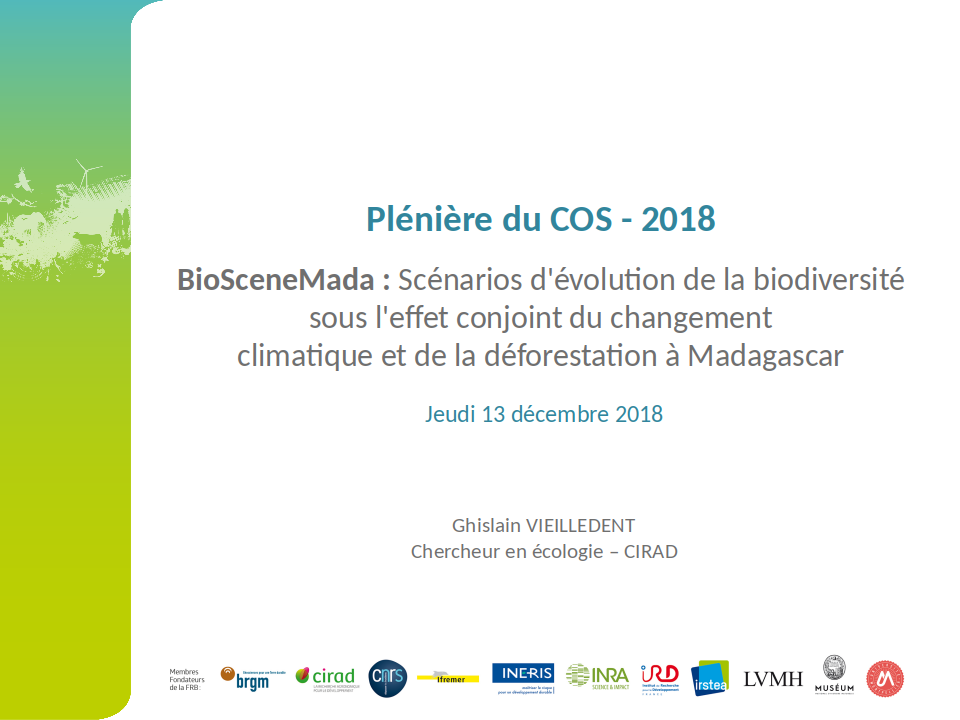
\includegraphics[height=\paperheight,width=\paperwidth]{figs/Masque.png}
%   }
%   \setbeamertemplate{navigation symbols}{}
%   % Remove shadow from block
%   \setbeamertemplate{blocks}[rounded][shadow=false]
%   \begin{frame}[plain]
%   \end{frame}
% }

% Title page
{
  \setbeamertemplate{navigation symbols}{}
  \begin{frame}[plain, noframenumbering]
  \begin{center}
  \small{\textbf{FAO workshop -- Santa Marta (Colombia), July 2024}}
  \end{center}
  \vspace{-0.5cm}
  \titlepage % Presentation first page
  \vspace{-3cm}
  \begin{center}
    
\includegraphics[width=\textwidth]{figs/Barre_couleur}
    
    \vspace{0.25cm}
    
    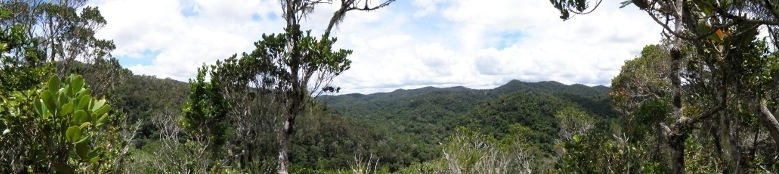
\includegraphics[width=10cm]{figs/Banniere}
    
    \small{Ghislain VIEILLEDENT$^{1}$\hspace{0.25cm}Thomas ARSOUZE$^{1}$\hspace{0.25cm}FAO team$^{2}$}
      
    \vspace{0.25cm}
    
    {\scriptsize
      \begin{tabular}{l}
        $[1]$ \textbf{Cirad} UMR AMAP, $[2]$ \textbf{FAO} Rome and Latin America
      \end{tabular}
    }
    
    
\includegraphics[width=0.8\textwidth]{figs/partners_logos}
    
  \end{center}
  \end{frame}
}

% %%%%%%%%%%%%%%%%%%%%%%%%%%%%%%%%%%%%%%%%%%%%%%%%%%%%%%%%%%%%%%%%

\placelogotrue
\begin{frame}
  \frametitle{Outline}
  \begin{columns}[c]
    \begin{column}{0.5\textwidth}
      \tableofcontents[sections=1]
      \vspace{0.5cm}
      \tableofcontents[sections=2]
      \vspace{0.5cm}
      \tableofcontents[sections=3]
    \end{column}
    \begin{column}{0.5\textwidth}
        \tableofcontents[sections=4]
        \vspace{0.5cm}
        \tableofcontents[sections=5]
    \end{column}
  \end{columns}
\end{frame}
\placelogofalse

\section{The deforisk QGIS plugin}
\label{sec:org9850c0d}

\subsection{Aim and specificities}
\label{sec:orgf11df72}

\begin{frame}[label={sec:org5ba602a}]{Aims}
\begin{itemize}
\item Provide \textbf{a tool} to create and compare \textbf{deforestation risk maps}.
\item At the \textbf{jurisdictional} level.
\item Following \textbf{Verra's methodology} for certification.
\item \textbf{Allocating deforestation} to projects within the jurisdiction.
\end{itemize}
\end{frame}

\begin{frame}[label={sec:orgf802a0a}]{Specificities}
\begin{itemize}
\item Open-source and Python based: transparency, reproducibility.
\item Computationally efficient:
\begin{itemize}
\item Processing raster by blocks.
\item Running tasks in parallel.
\end{itemize}
\item OS independent: Windows, Linux, MacOS.
\item Should run on any computer with average performance.
\item Performant alternative statistical models (iCAR).
\item Fully documented and translated (English, Spanish, French).
\item Help with data preparation.
\item Should be (relatively) easy to use.
\end{itemize}
\end{frame}

\begin{frame}[label={sec:orgc281ac2},fragile]{Python based}
 The \texttt{deforisk} plugin relies on four Python packages developed specifically for modelling deforestation:

\begin{itemize}
\item \texttt{geefcc}: make forest cover change maps from Google Earth Engine (GEE).
\item \texttt{pywdpa}: downloading protected areas from the World Database on Protected Areas (WDPA).
\item \texttt{forestatrisk}: model deforestation and predict the spatial deforestation.
\item \texttt{riskmapjnr}: risk maps following Verra JNR methodologies.
\end{itemize}

\begin{center}
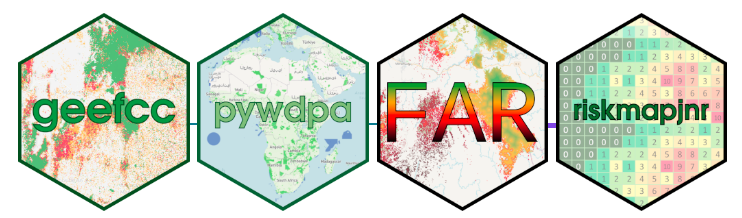
\includegraphics[width=0.7\textwidth]{figs/logos-packages.png}
\end{center}
\end{frame}

\begin{frame}[label={sec:orgf1660cc},fragile]{Processing raster by blocks}
 \begin{itemize}
\item Raster files of forest cover change and explanatory variables might occupy a space of several gigabytes on disk.
\item Processing such large rasters in memory can be prohibitively intensive on computers with limited RAM.
\item Functions used in the \texttt{deforisk} plugin process large rasters by blocks of pixels representing subsets of the raster data.
\item This makes computation efficient, with low memory usage.
\end{itemize}

\begin{center}
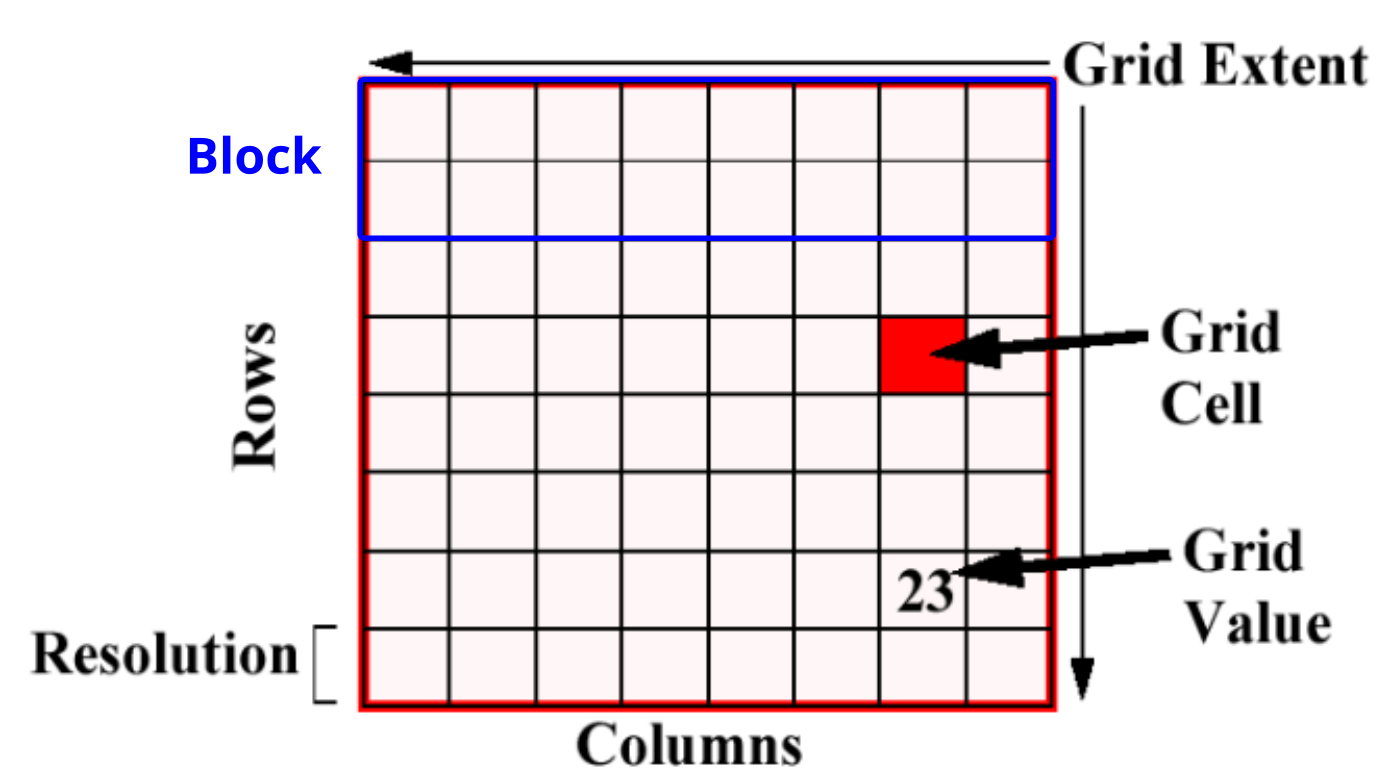
\includegraphics[width=6cm]{figs/raster_block.png}
\end{center}
\end{frame}

\begin{frame}[label={sec:org6dbff18},fragile]{Running tasks in parallel}
 \begin{itemize}
\item State-of-the-art approach to select the best risk map implies repeating tasks (model, periods).
\item To save computation time, the \texttt{deforisk} plugin use the QGIS task manager.
\item Allows running several analysis in parallel.
\end{itemize}

\vspace{0.25cm}

\begin{center}
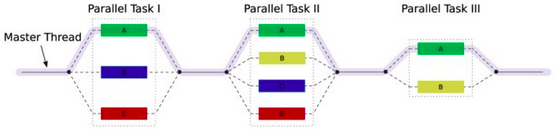
\includegraphics[width=9cm]{figs/parallel_tasks.png}
\end{center}
\end{frame}

\subsection{Website and documentation}
\label{sec:org7f2ce28}

\begin{frame}[label={sec:org6c026ea}]{Website and documentation}
The website includes all the documentation to use the plugin:

\begin{itemize}
\item \href{https://deforisk-qgis-plugin/installation.html}{Installation page}: How to install the plugin?
\item \href{https://deforisk-qgis-plugin/plugin\_api.html}{Plugin API page}: What is the meaning of each parameter?
\item \href{https://deforisk-qgis-plugin/get\_started.html}{Get started page}. How to start using the plugin on a small area of interest?
\item \href{https://deforisk-qgis-plugin/articles.html}{Articles' page}. How can I use the plugin for specific cases (subnational jurisdictions, user's data)?
\item \href{https://deforisk-qgis-plugin.org/articles/references.html}{References' page}: A page with reference documents including presentations.
\end{itemize}

\begin{columns}
\begin{column}{0.5\columnwidth}
\flushright \url{https://deforisk-qgis-plugin.org}
\end{column}
\begin{column}{0.5\columnwidth}
\begin{center}
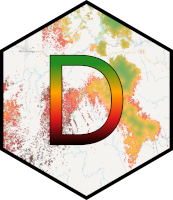
\includegraphics[width=2cm]{figs/logo-deforisk.png}
\end{center}
\end{column}
\end{columns}
\end{frame}

\subsection{Installation}
\label{sec:orgfff0012}

\begin{frame}[label={sec:org7337406},fragile]{Installation}
 Reduced number of steps for installing the plugin:

\begin{itemize}
\item Install QGIS and GDAL on you system (using \texttt{OSGeo4W} on Windows).
\item Install the \texttt{forestatrisk} and \texttt{riskmapjnr} Python packages using pip.
\item \href{https://github.com/ghislainv/deforisk-qgis-plugin/archive/refs/heads/main.zip}{Download} and install the \texttt{deforisk} plugin from QGIS.
\item (Unix-like systems only: install OSM tools).
\end{itemize}

\begin{center}
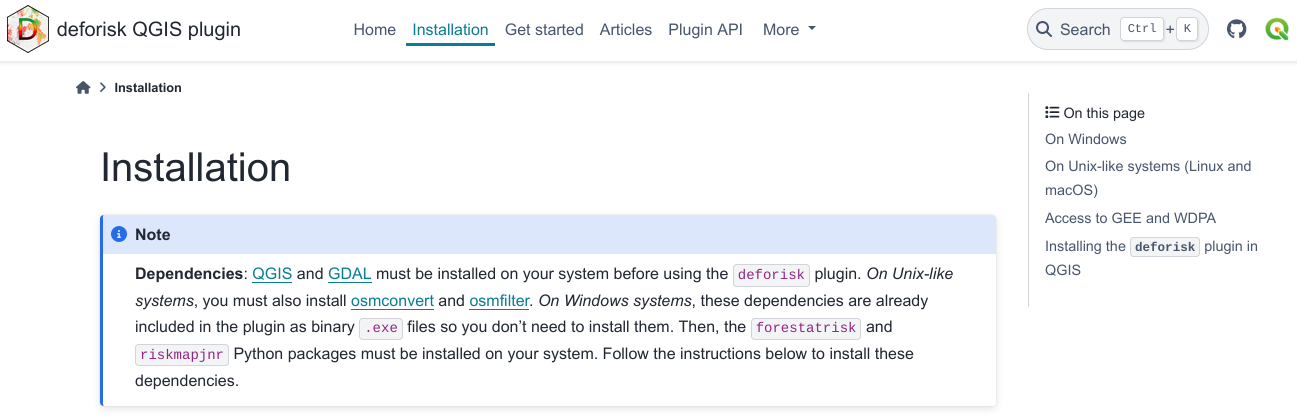
\includegraphics[width=0.9\textwidth]{figs/installation.png}
\end{center}
\end{frame}

\section{Data preparation}
\label{sec:org075a2c7}

\subsection{Get variables}
\label{sec:org9703005}

\begin{frame}[label={sec:orgb3013e4}]{Get variables}
\begin{columns}
\begin{column}{0.5\columnwidth}
\begin{itemize}
\item Functions to help prepare the data for modelling deforestation.
\item Two different sources for \textbf{forest cover change} (GFC or TMF).
\item Spatial explanatory variables describing \textbf{forest accessibility} and
\textbf{land tenure} (altitude, slope, distance to roads, protected areas, etc.).
\end{itemize}
\end{column}

\begin{column}{0.5\columnwidth}
\begin{center}
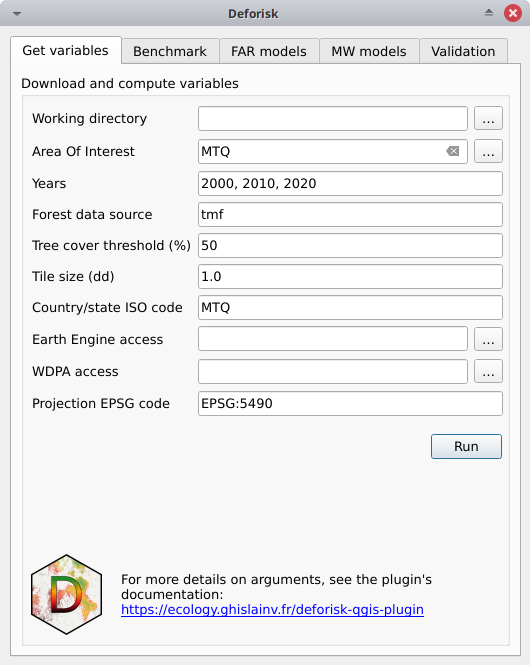
\includegraphics[width=5cm]{figs/plugin_api/interface_variables.png}
\end{center}
\end{column}
\end{columns}
\end{frame}

\subsection{Forest cover change data}
\label{sec:orgcf5ecd8}

\begin{frame}[label={sec:org67ec52b}]{GFC dataset}
\begin{itemize}
\item Hansen et al. 2013.
\item Global dataset encompassing all forest types.
\item Tree cover and annual tree cover loss.
\item 30m resolution, from 2000 on.
\item Data: \url{https://glad.earthengine.app/view/global-forest-change}
\end{itemize}

\begin{center}
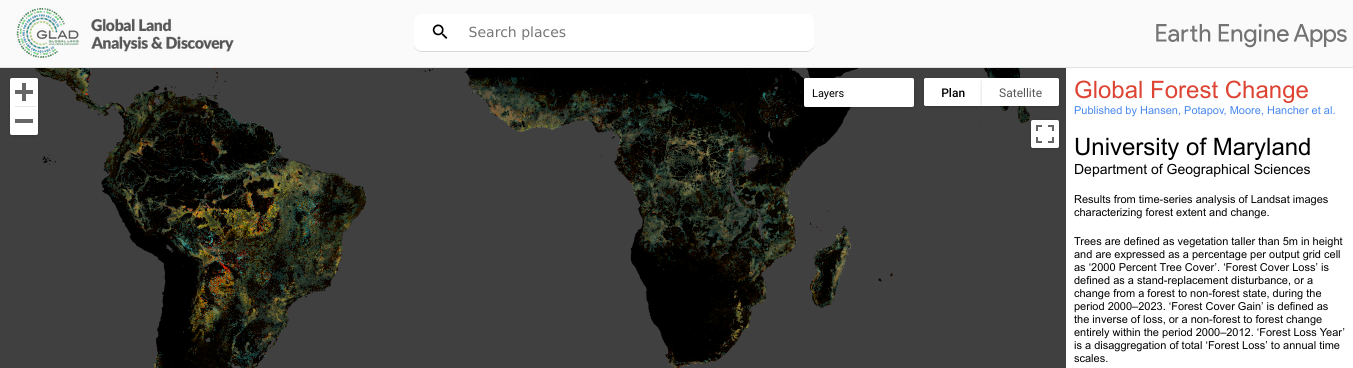
\includegraphics[width=\textwidth]{figs/gfc.png}
\end{center}
\end{frame}

\begin{frame}[label={sec:org3cd736c}]{TMF dataset}
\begin{itemize}
\item Vancutsem et al. 2021.
Tropical Moist Forests (evergreen forest, no dry deciduous forests).
\item 30m resolution, from 1990 on.
\item Tropical deforestation was underestimated (-33\% in 2000--2012, Hansen
et al. 2013), especially in Africa.
\item Data: \url{https://forobs.jrc.ec.europa.eu/TMF/}.
\end{itemize}

\vspace{0.25cm}

\begin{center}
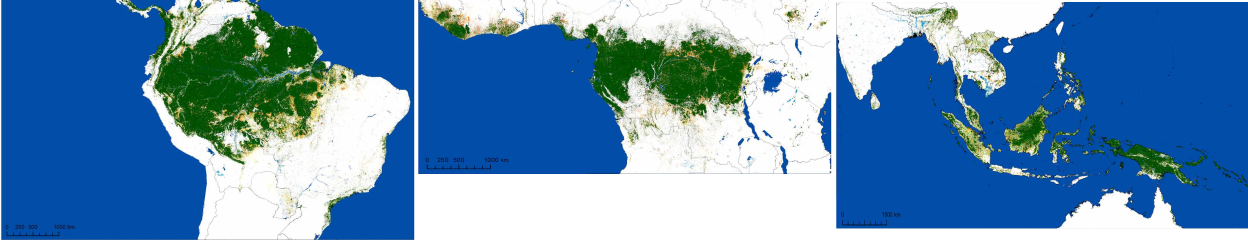
\includegraphics[width=\textwidth]{figs/Vancutsem2021-maps-wide.png}
\end{center}
\end{frame}

\begin{frame}[label={sec:orgae8b85b}]{TMF dataset}
\begin{itemize}
\item Precise enough to visually identify the causes of deforestation
(logging, fires, agriculture)
\end{itemize}

\begin{center}
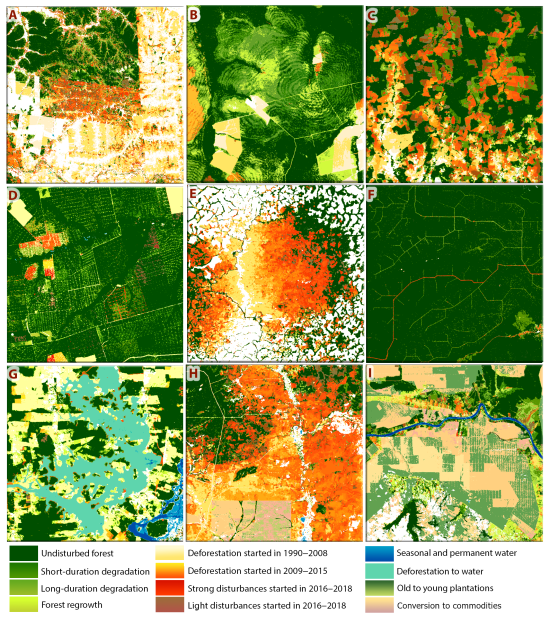
\includegraphics[width=0.5\textwidth]{figs/Vancutsem2021-patterns.png}
\end{center}
\end{frame}

\subsection{Spatial explanatory variables}
\label{sec:org75f280d}

\begin{frame}[label={sec:orgaac5087}]{Spatial variables}
The plugin helps computing height explanatory variables.

\begin{center}
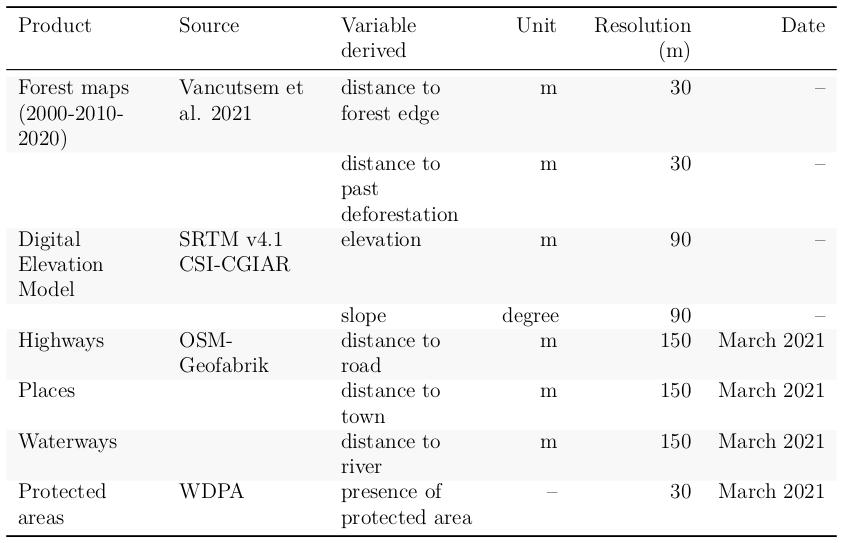
\includegraphics[width=0.75\textwidth]{figs/variables-tab.png}
\end{center}
\end{frame}

\begin{frame}[label={sec:orgfdeaa52}]{Spatial variables}
\begin{center}
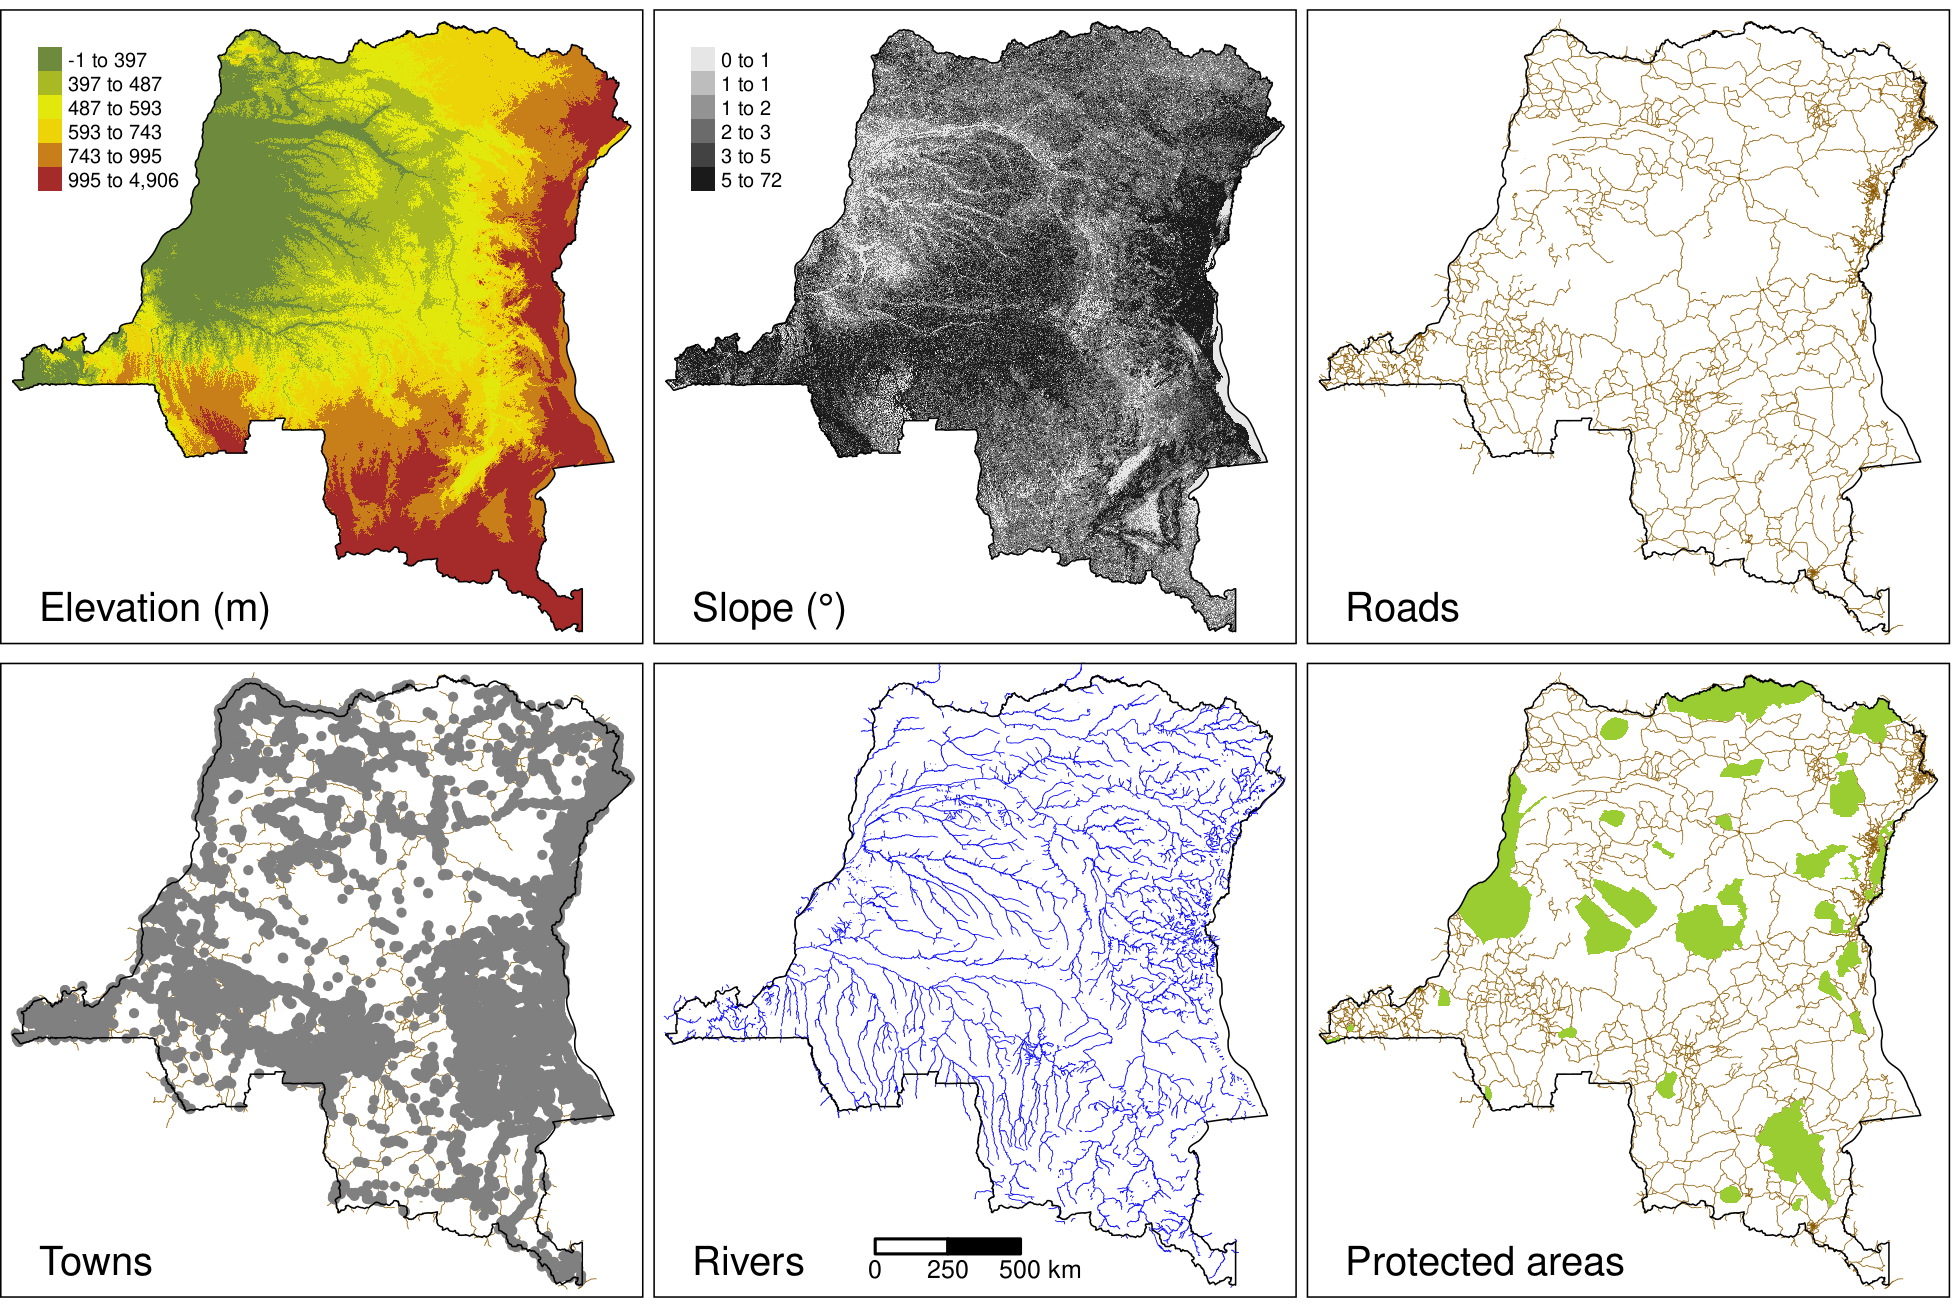
\includegraphics[width=0.8\textwidth]{figs/sm/var.png}
\end{center}

\centering \textbf{Spatial explanatory variables in DRC}
\end{frame}

\begin{frame}[label={sec:orgbad9b56}]{Roads}
\begin{itemize}
\item OpenStreetMap (OSM)
\item ``motorway'', ``trunk'', ``primary'', ``secondary'' and ``tertiary'' roads
\item 3.6 million roads from OSM
\end{itemize}

\begin{center}
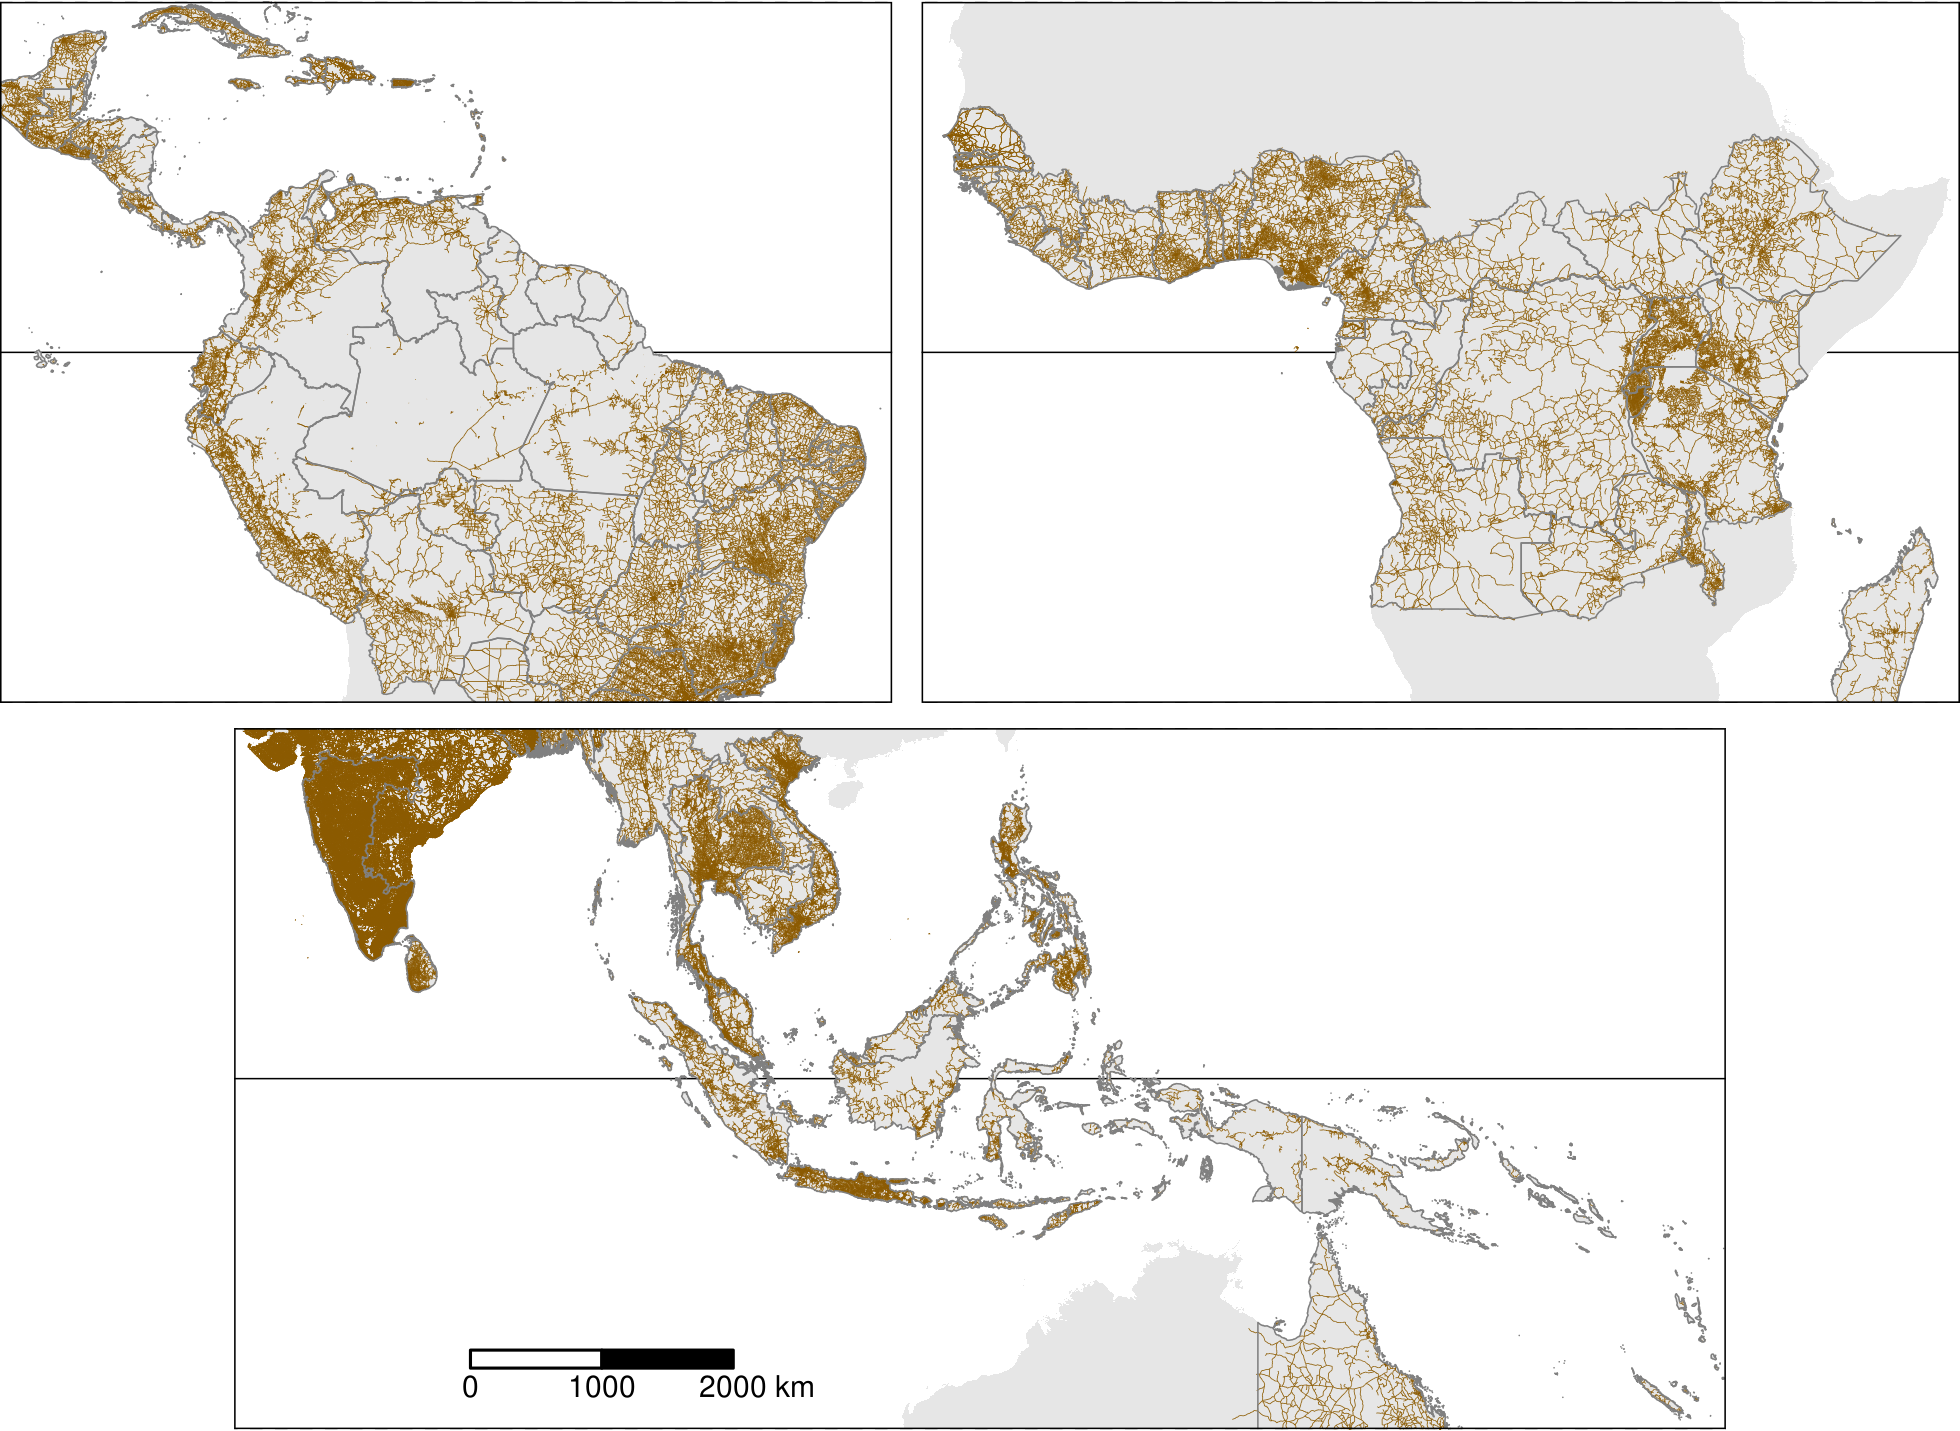
\includegraphics[width=0.7\textwidth]{figs/sm/roads.png}
\end{center}
\end{frame}

\begin{frame}[label={sec:org11e2e7c}]{Protected areas}
\begin{itemize}
\item PA status: ``Designated'', ``Inscribed'', ``Established'', or ``Proposed''.
\item 85,000 protected areas from WDPA.
\end{itemize}

\begin{center}
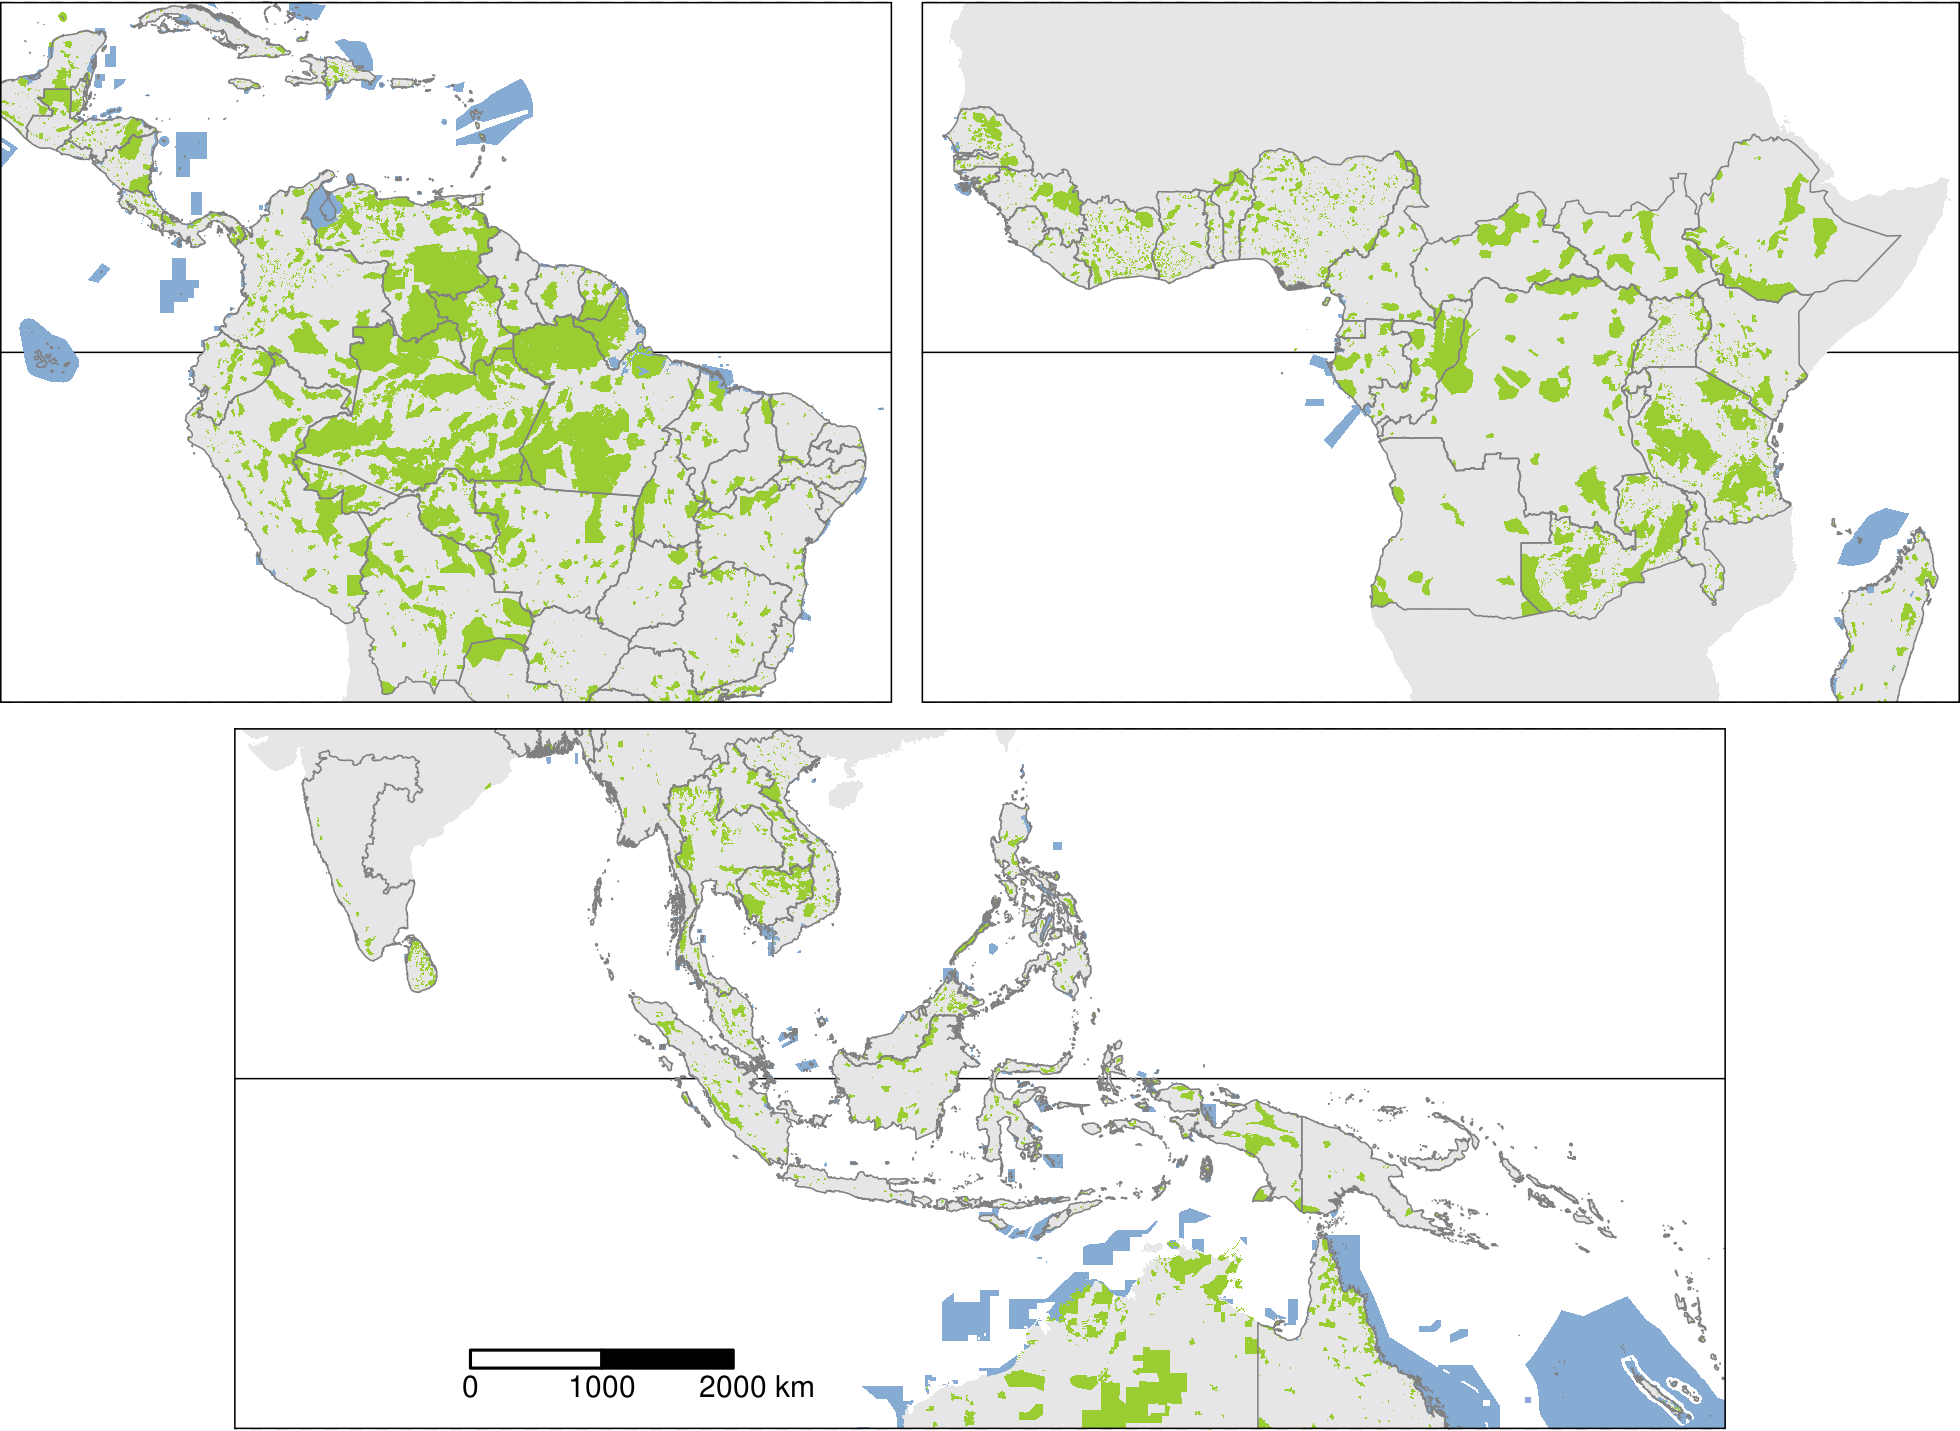
\includegraphics[width=0.7\textwidth]{figs/sm/pa.png}
\end{center}
\end{frame}

\section{Models and validation}
\label{sec:orgb92fcc6}

\subsection{Benchmark model}
\label{sec:org6ebc96a}

\begin{frame}[label={sec:org2e32298}]{Benchmark model}
\begin{columns}
\begin{column}{0.5\columnwidth}
\begin{itemize}
\item Benchmark model or reference model.
\item A reasonably good deforestation model (better than a null model).
\item Assuming a \emph{decrease of deforestation with distance to forest edge} (commonly admitted).
\item And a \emph{different model between subjurisdictions} (regional variability).
\item See presentation \textbf{Cirad and FAO}. 2024. \href{https://deforisk-qgis-plugin.org/\_static/references/Cirad2024-riskmap-verra.pdf}{Jurisdictional risk maps for allocating deforestation}.
\end{itemize}
\end{column}

\begin{column}{0.5\columnwidth}
\begin{center}
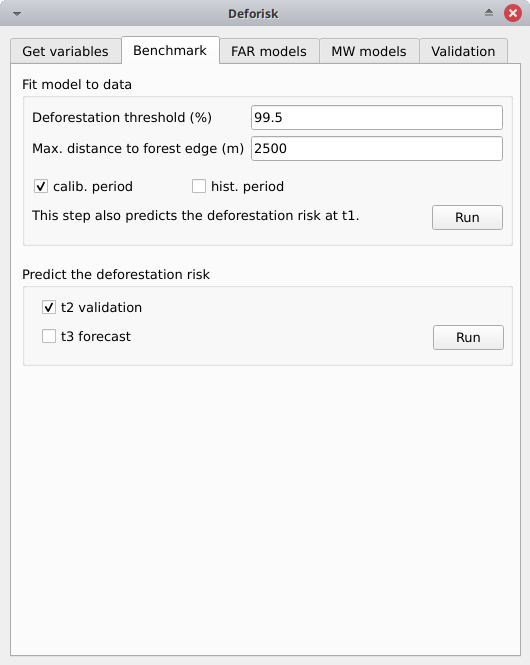
\includegraphics[width=5cm]{figs/plugin_api/interface_benchmark.png}
\end{center}  
\end{column}
\end{columns}
\end{frame}

\subsection{Forestatrisk models}
\label{sec:org63e7522}

\begin{frame}[label={sec:orgefdba21}]{Forestatrisk models}
\begin{columns}
\begin{column}{0.5\columnwidth}
\begin{itemize}
\item Three statistical models: iCAR, GLM, RF.
\item iCAR: Logistic regression with spatial random effects (iCAR process).
\item GLM: Generalized Linear Model, simple logistic regression (no random effects).
\item Random Forest model: random regression trees.
\item Statistical models based on a sample of the observations.
\end{itemize}
\end{column}

\begin{column}{0.5\columnwidth}
\begin{center}
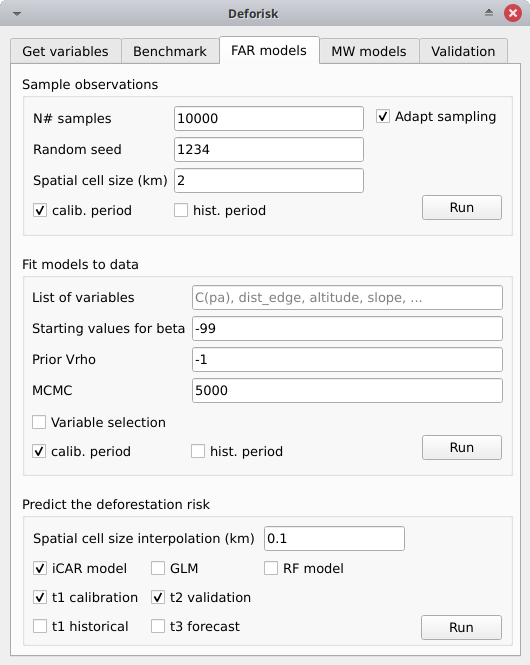
\includegraphics[width=5cm]{figs/plugin_api/interface_far_models.png}
\end{center}  
\end{column}
\end{columns}
\end{frame}

\begin{frame}[label={sec:org073c55e}]{Sampling for FAR models}
\begin{itemize}
\item We consider the forest cover change between \(t\) and \(t+1\).
\item Stratified sampling between deforested/non-deforested pixels.
\item Total number of points proportional to the forest cover (from
20,000 to 100,000 points per study area).
\end{itemize}

\begin{center}
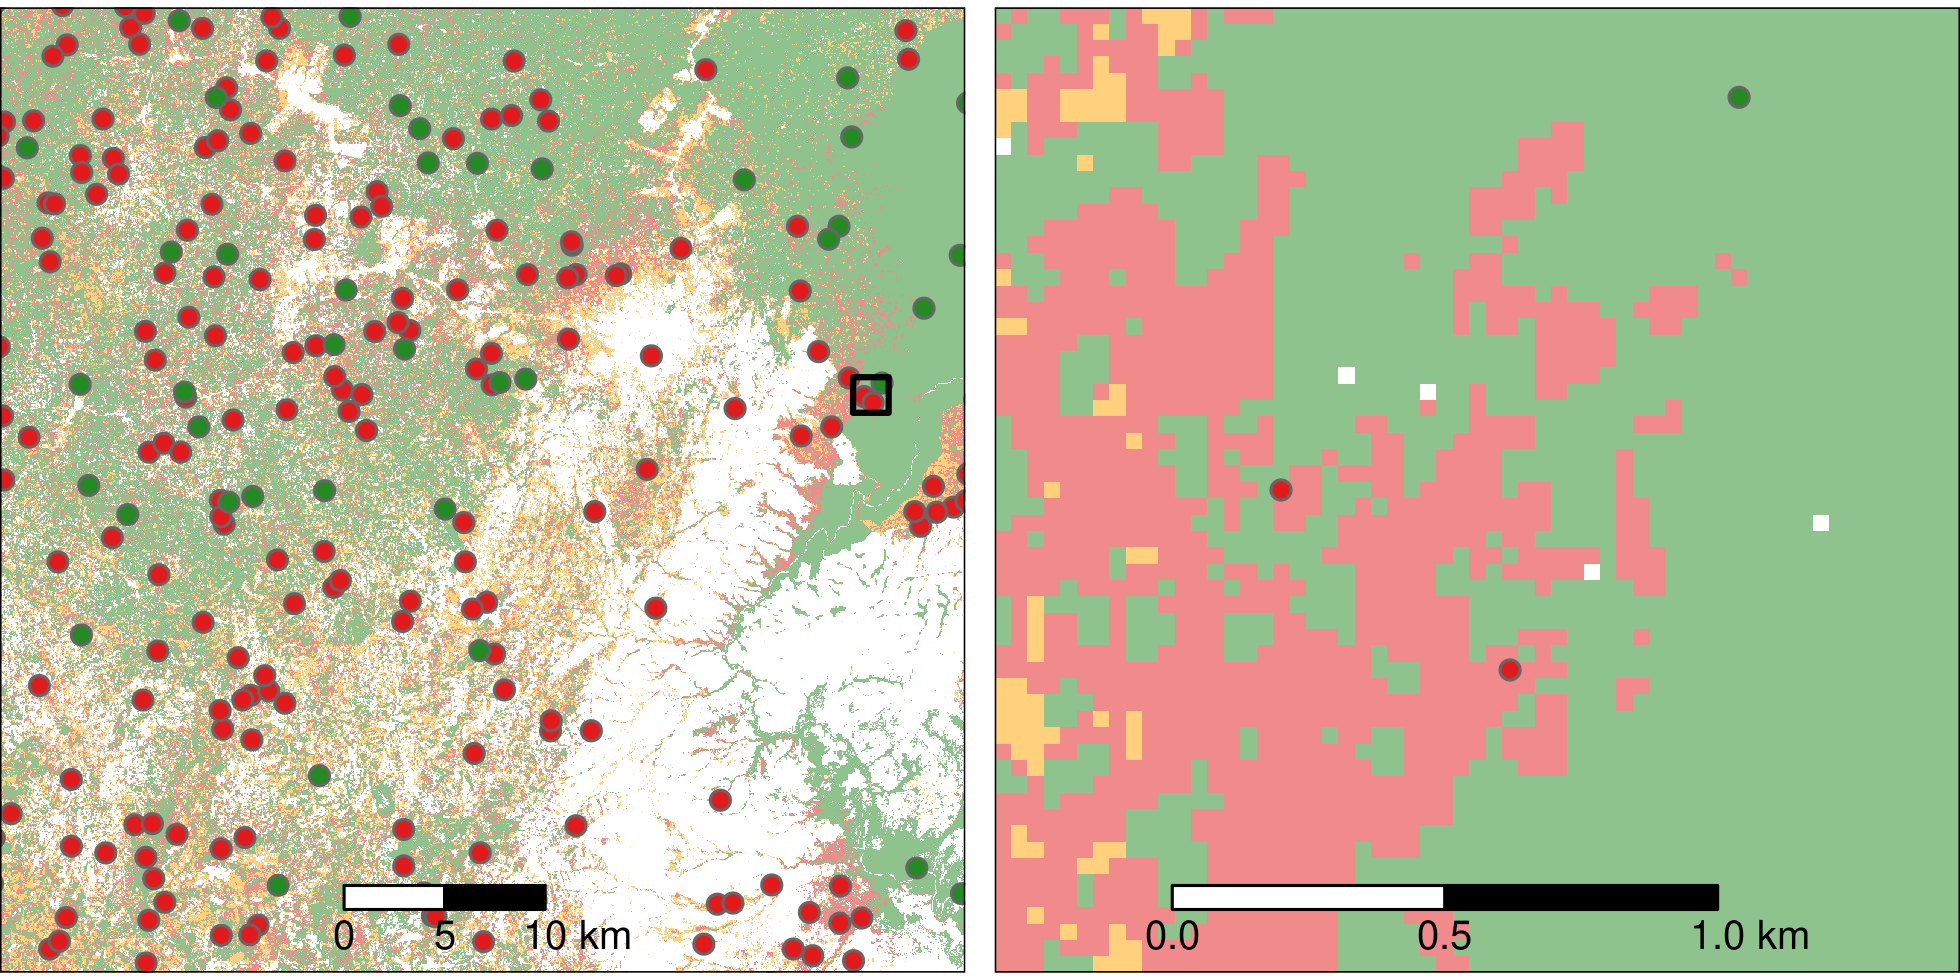
\includegraphics[width=0.7\textwidth]{figs/sm/sample.png}
\end{center}
\end{frame}

\begin{frame}[label={sec:org165f56f}]{iCAR model}
\begin{columns}
\begin{column}{0.5\columnwidth}
A logistic regression model with iCAR process:

\begin{equation*}
\begin{split}
  y_i \sim \mathcal{B}ernoulli(\theta_i)\\
  \text{logit}(\theta_i) = \alpha + X_i \beta + \rho_{j(i)}\\
  \rho_{j(i)} \sim \mathcal{N}ormal(\sum_{j^{\prime}} \rho_{j^{\prime}} / n_j,V_{\rho} / n_j)
\end{split}
\end{equation*}

\textbf{Random effects \(\rho_{j(i)}\) allows accounting for residual spatial variation not taken into account by model variables \(X_i\).}
\end{column}

\begin{column}{0.5\columnwidth}
\begin{center}
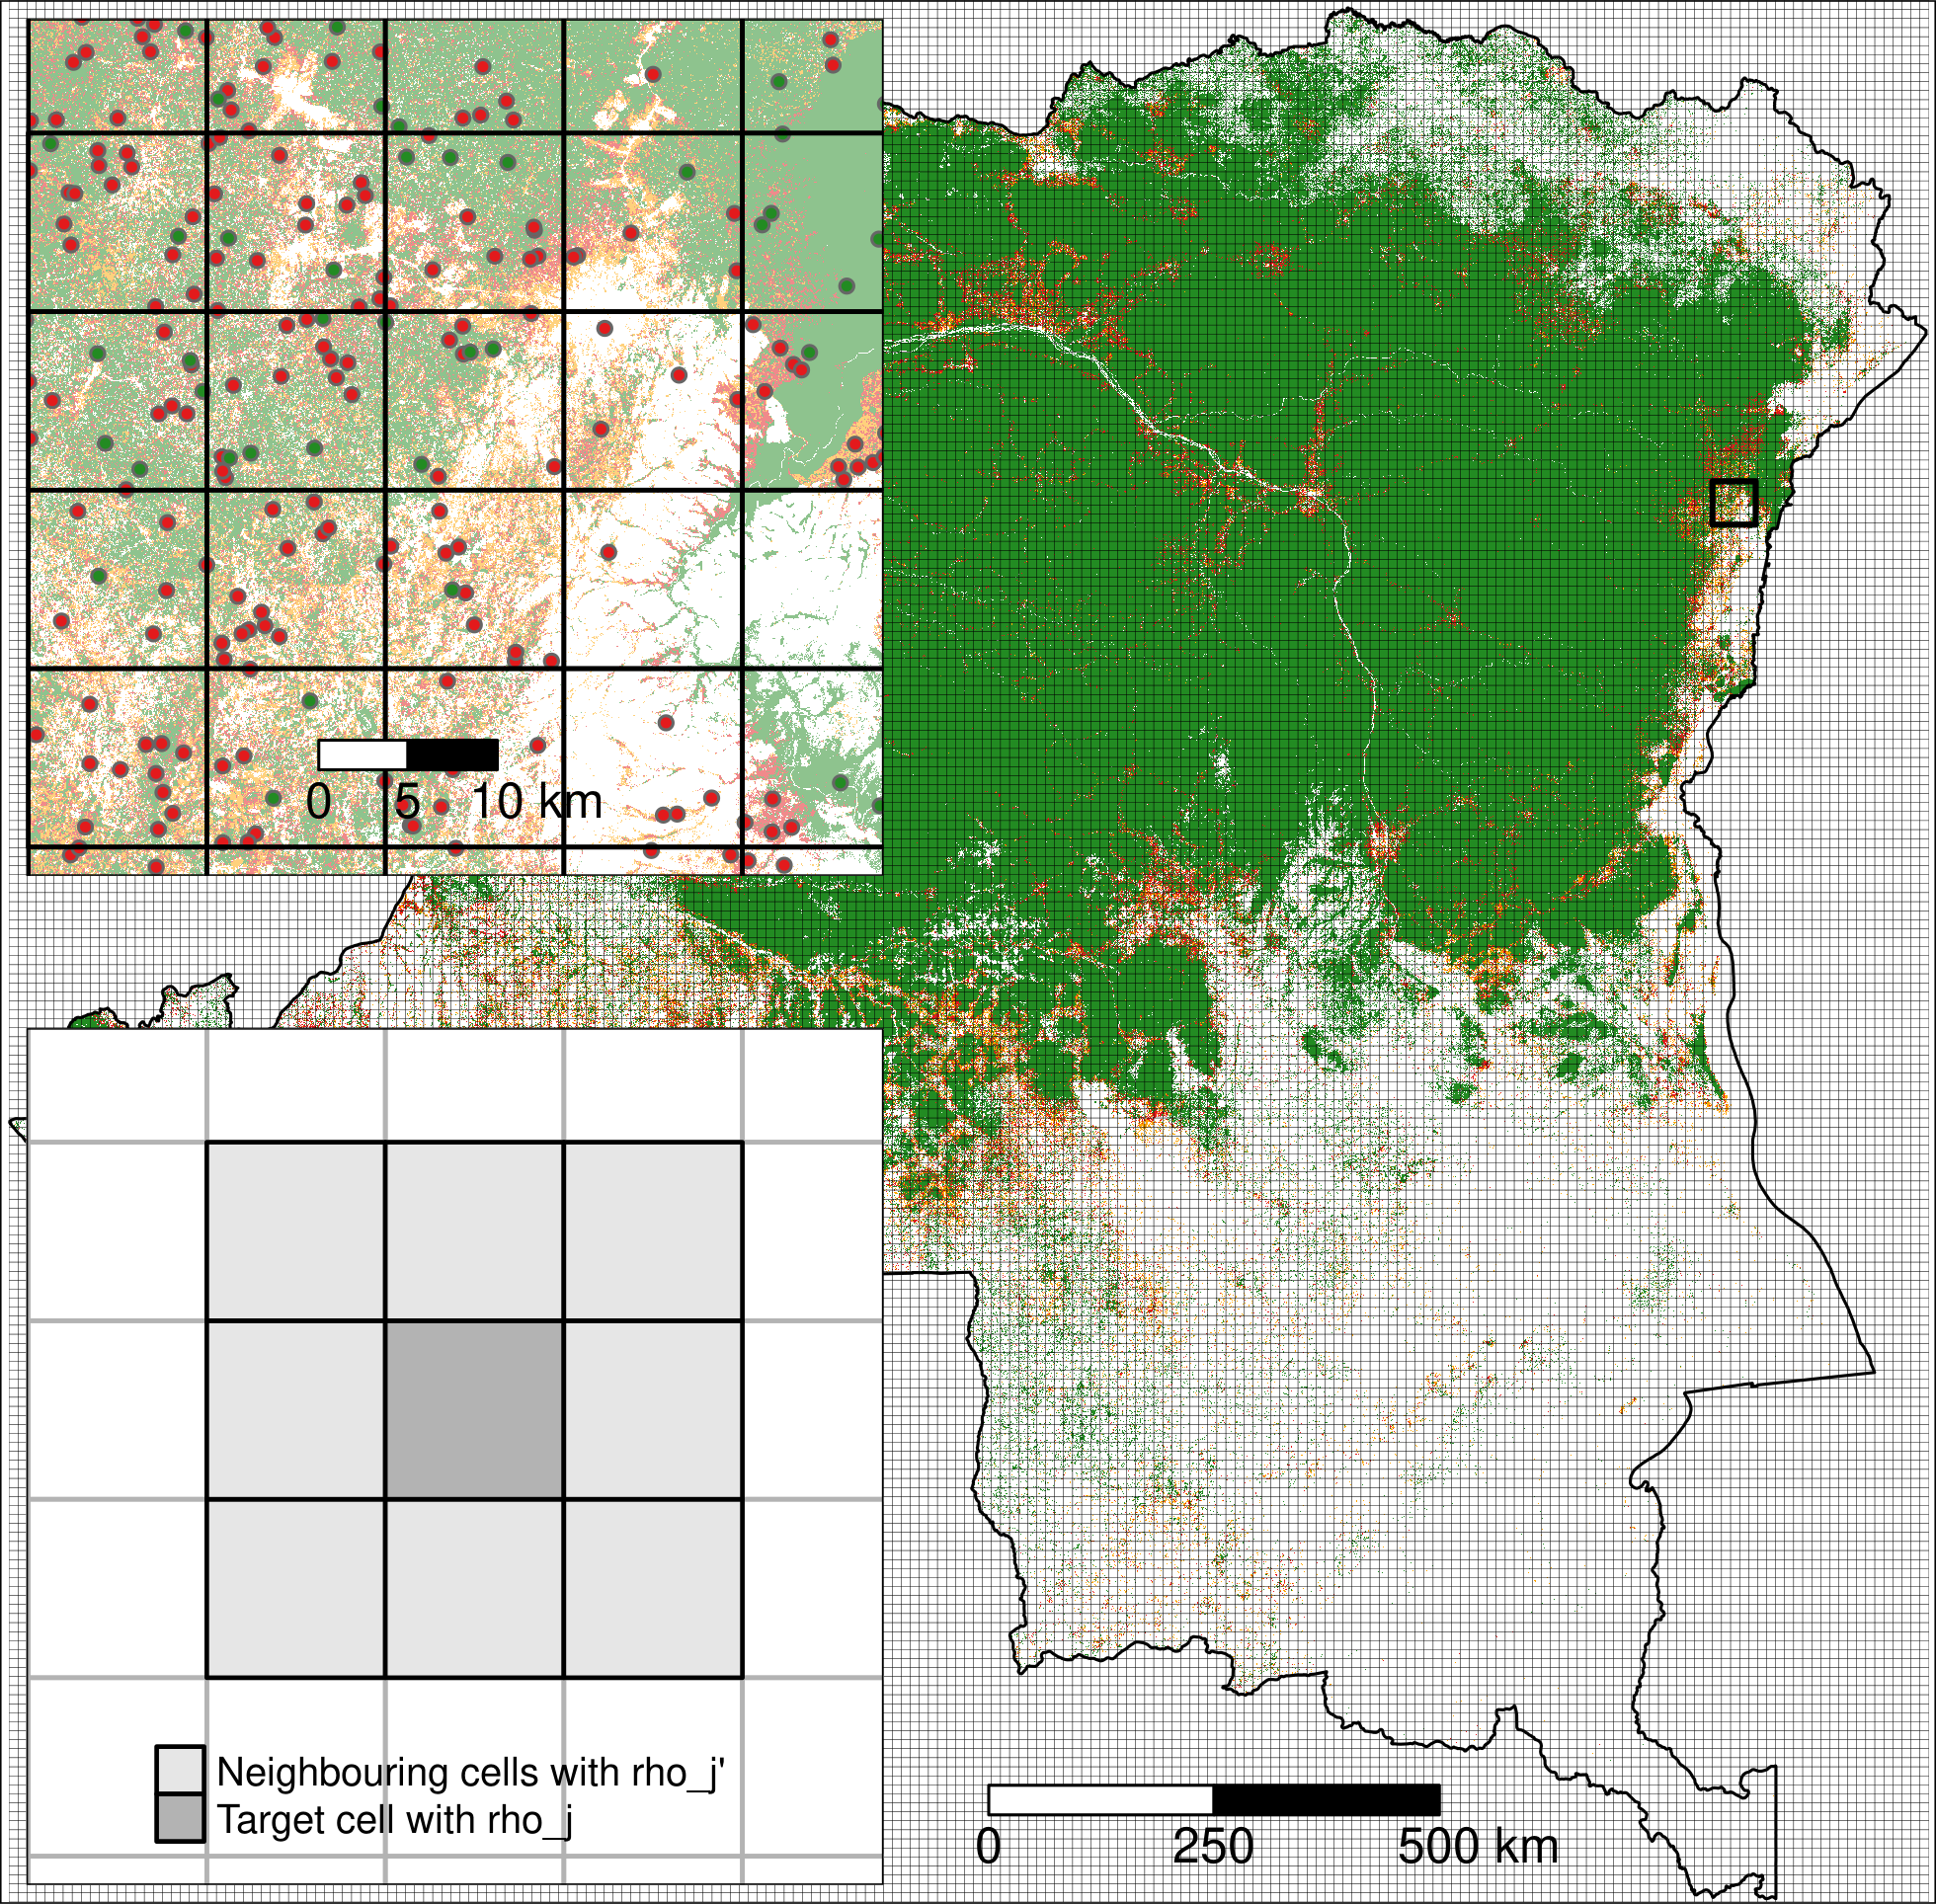
\includegraphics[width=\textwidth]{figs/sm/grid.png}
\end{center}

\centering \textbf{Square grid of 10km cells over DRC}
\end{column}
\end{columns}
\end{frame}

\begin{frame}[label={sec:org1ad1a41}]{Spatial random effects}
\begin{center}
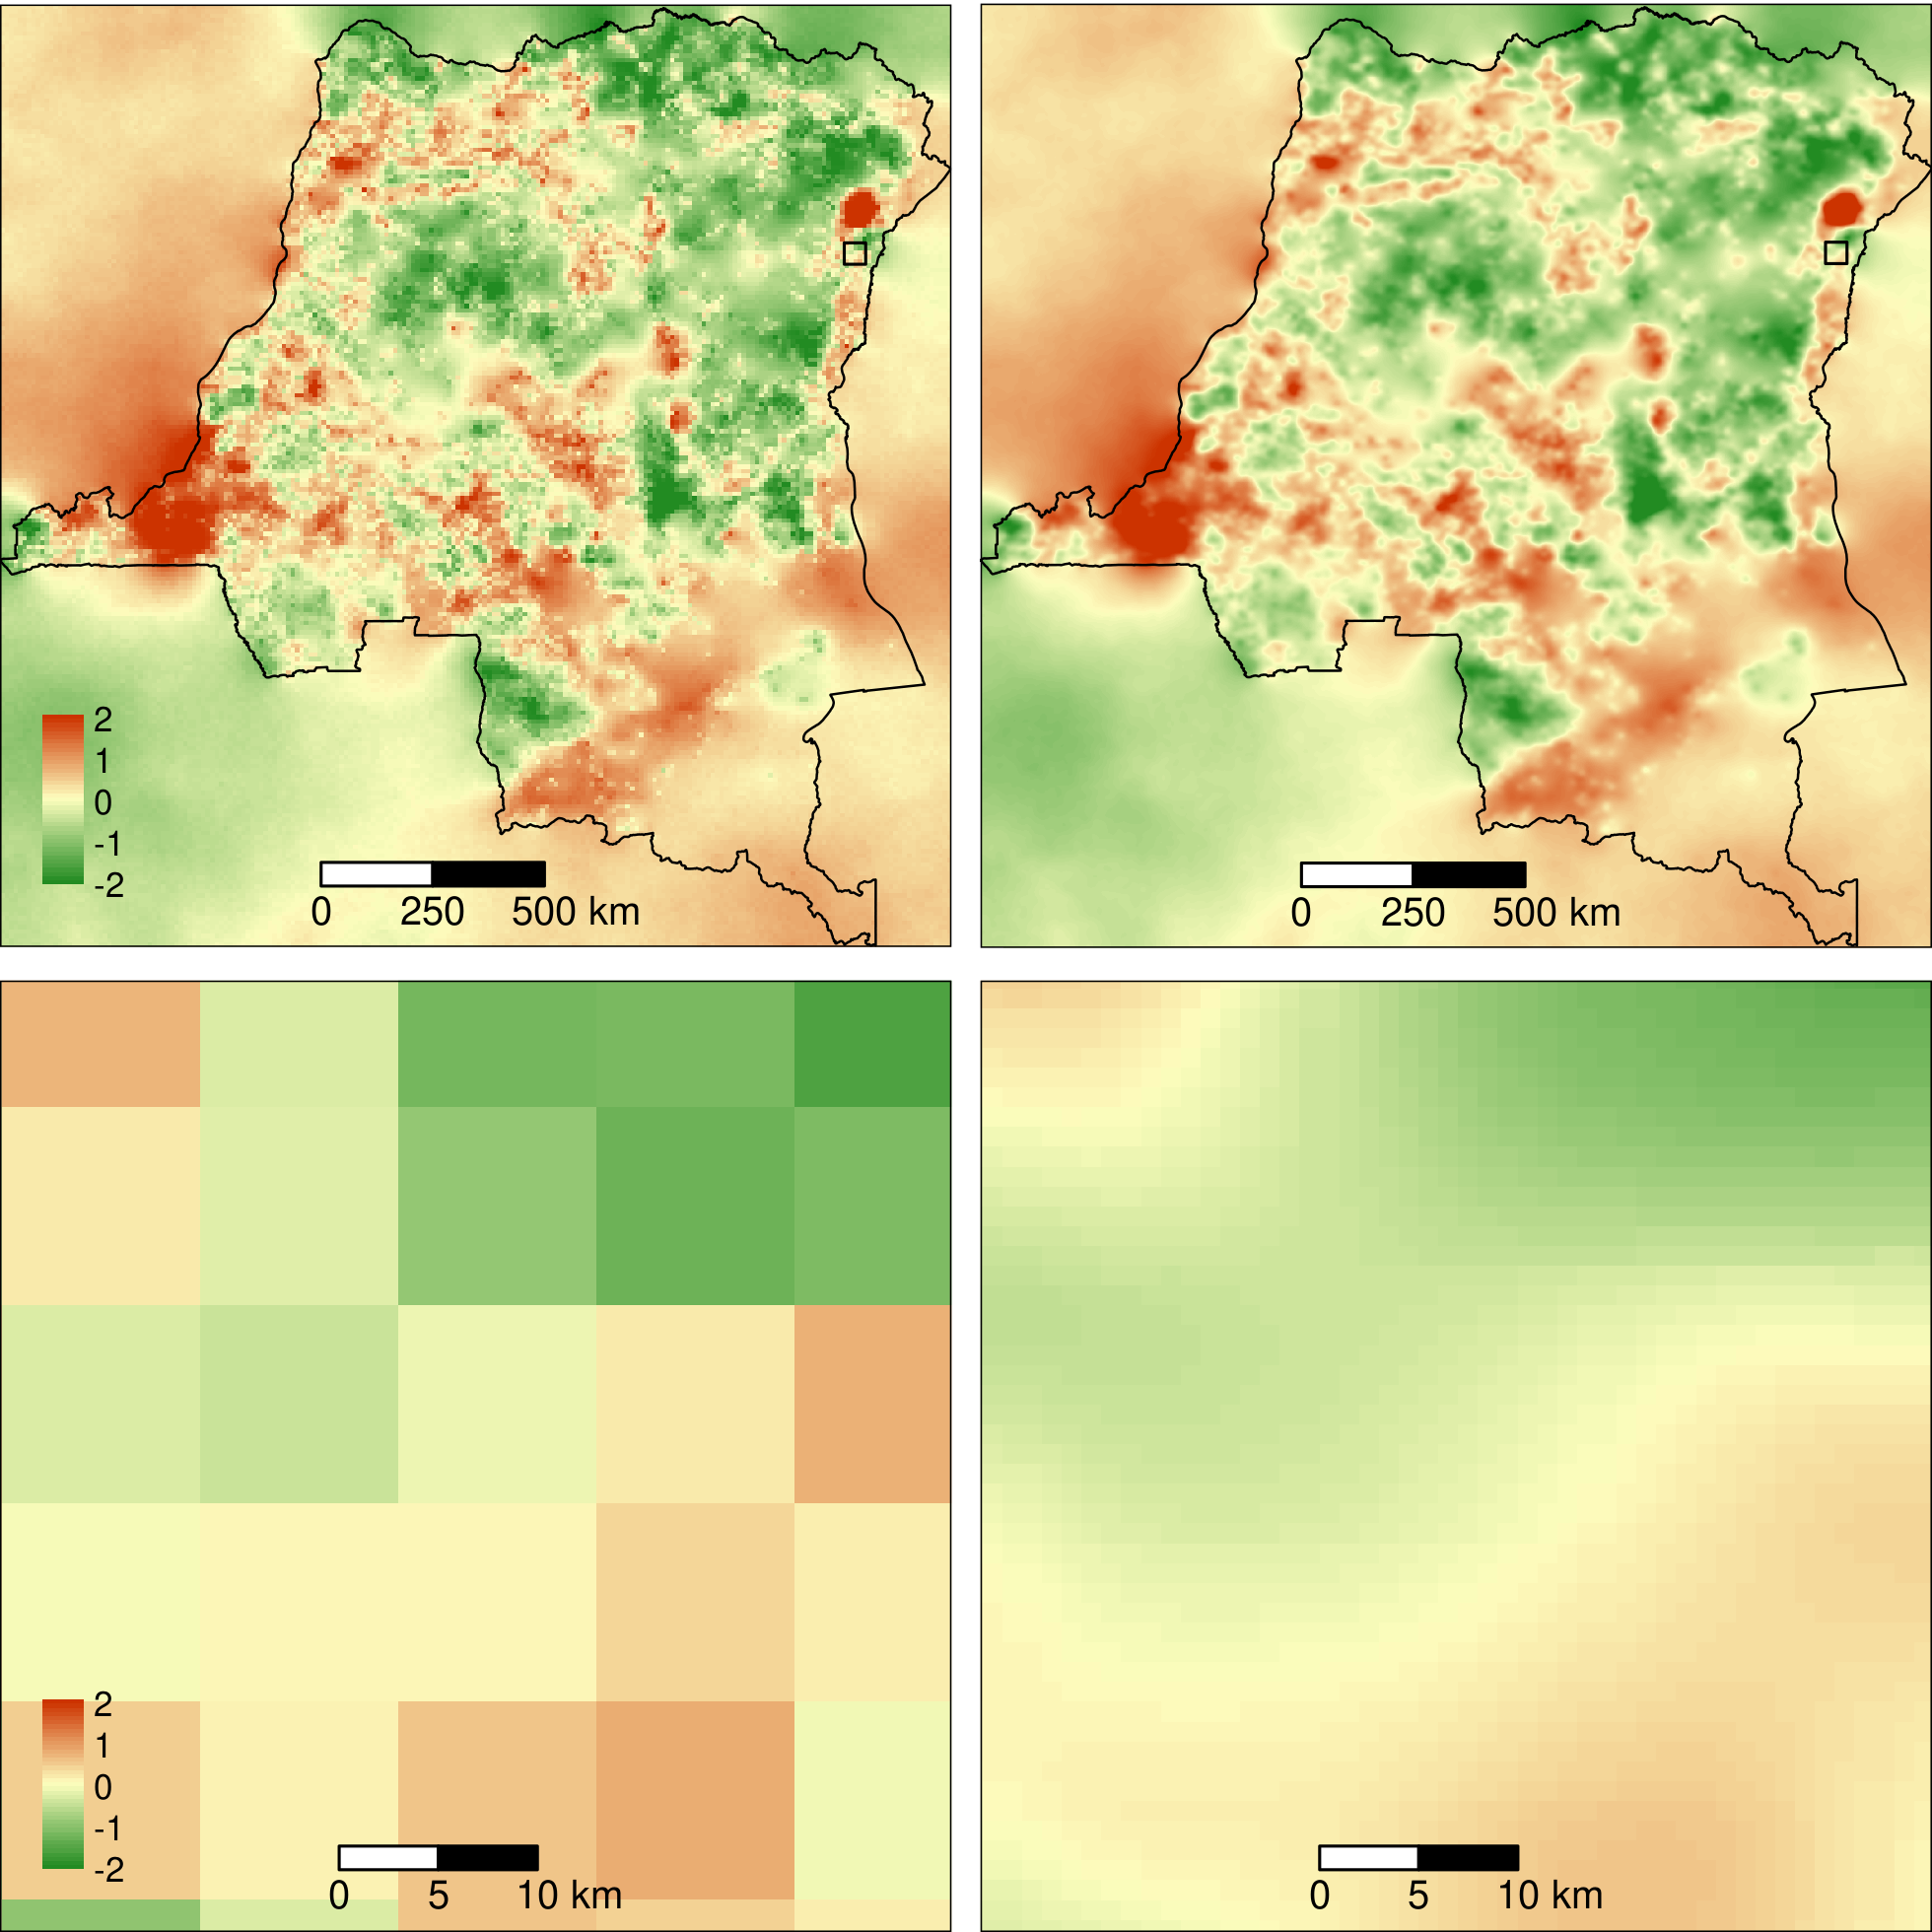
\includegraphics[width=0.6\textwidth]{figs/sm/rho.png}
\end{center}

\centering \textbf{Interpolation of spatial random effects at 1km in DRC}
\end{frame}

\begin{frame}[label={sec:orgfcc2a82}]{Spatial probability of deforestation}
\begin{itemize}
\item We use the fitted model to compute the spatial probability of
\end{itemize}
deforestation.
\begin{itemize}
\item Probabilities in [0, 1] are transformed into classes in [1, 65535].
\end{itemize}

\begin{center}
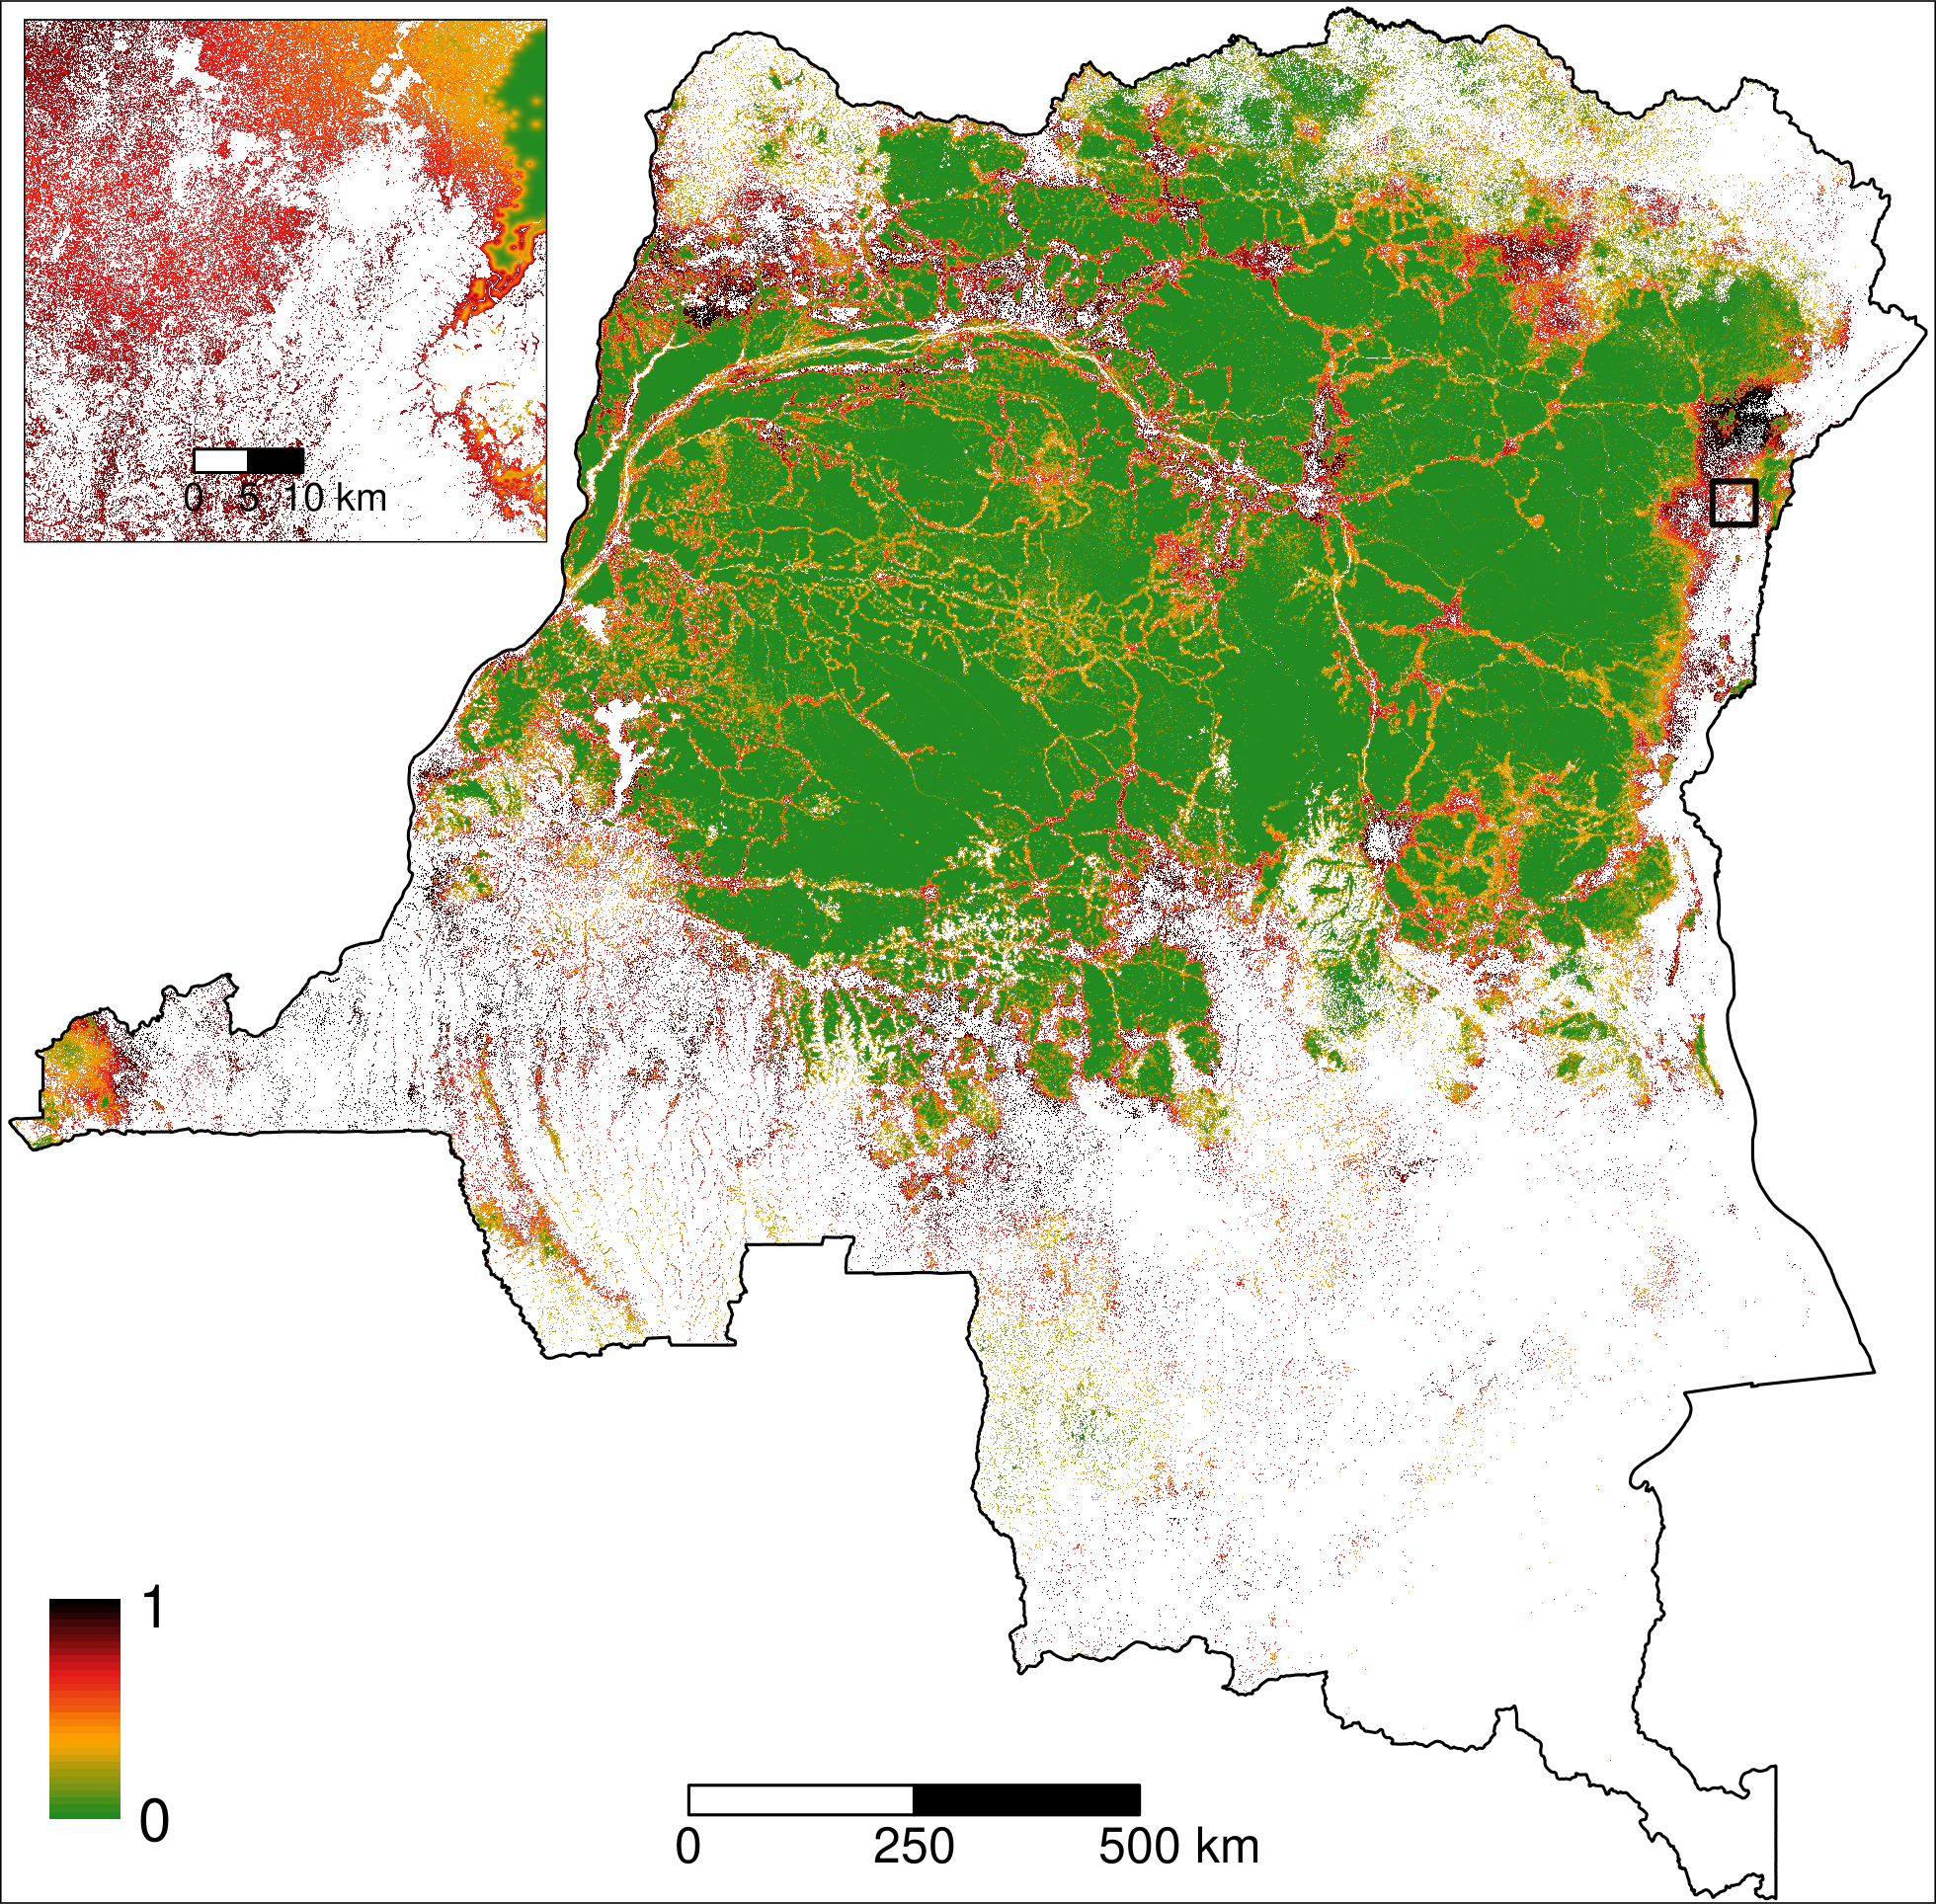
\includegraphics[width=0.5\textwidth]{figs/sm/prob.png}
\end{center}

\centering \textbf{Relative spatial probability of deforestation in DRC}
\end{frame}

\begin{frame}[label={sec:org2ef0ac7}]{GLM model}
A simple logistic regression model without random effects:

\begin{equation*}
\begin{split}
  y_i \sim \mathcal{B}ernoulli(\theta_i)\\
  \text{logit}(\theta_i) = \alpha + X_i \beta
\end{split}
\end{equation*}

Easy to compare with iCAR to see the impact of spatial random effects.
\end{frame}

\begin{frame}[label={sec:orgbf834e3}]{Random Forest model}
\begin{itemize}
\item Random Forest is an ensemble machine learning algorithm.
\item Combines multiple decision trees to create a more robust and accurate predictive model.
\end{itemize}

\begin{center}
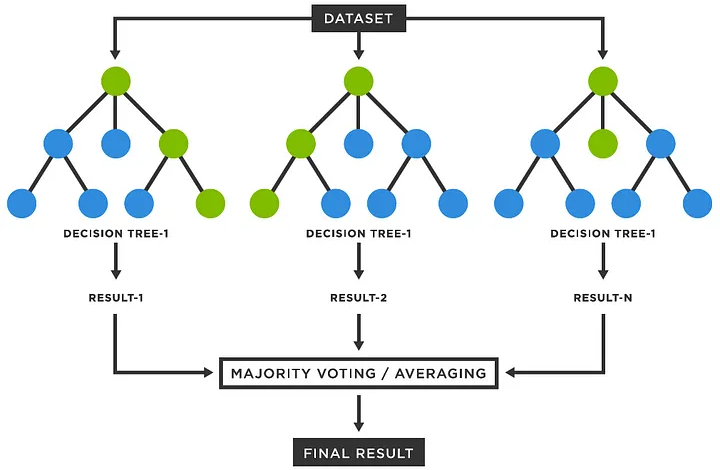
\includegraphics[width=0.7\textwidth]{figs/random_forest.png}
\end{center}
\end{frame}

\begin{frame}[label={sec:org6854c2d}]{ForestAtRisk in the tropics}
\begin{itemize}
\item \textbf{i.} Consider tropical moist forest in \textbf{92} countries (119 study areas)
\item \textbf{ii.} Estimate the current deforestation rate and uncertainty in each country
\item \textbf{iii.} Model the spatial risk of deforestation from environmental factors
\item \textbf{iv.} Forecast the deforestation assuming a business-as-usual scenario
\item \textbf{v.} Consequences in terms of carbon emissions
\end{itemize}

\vspace{0.5cm}
\begin{center}
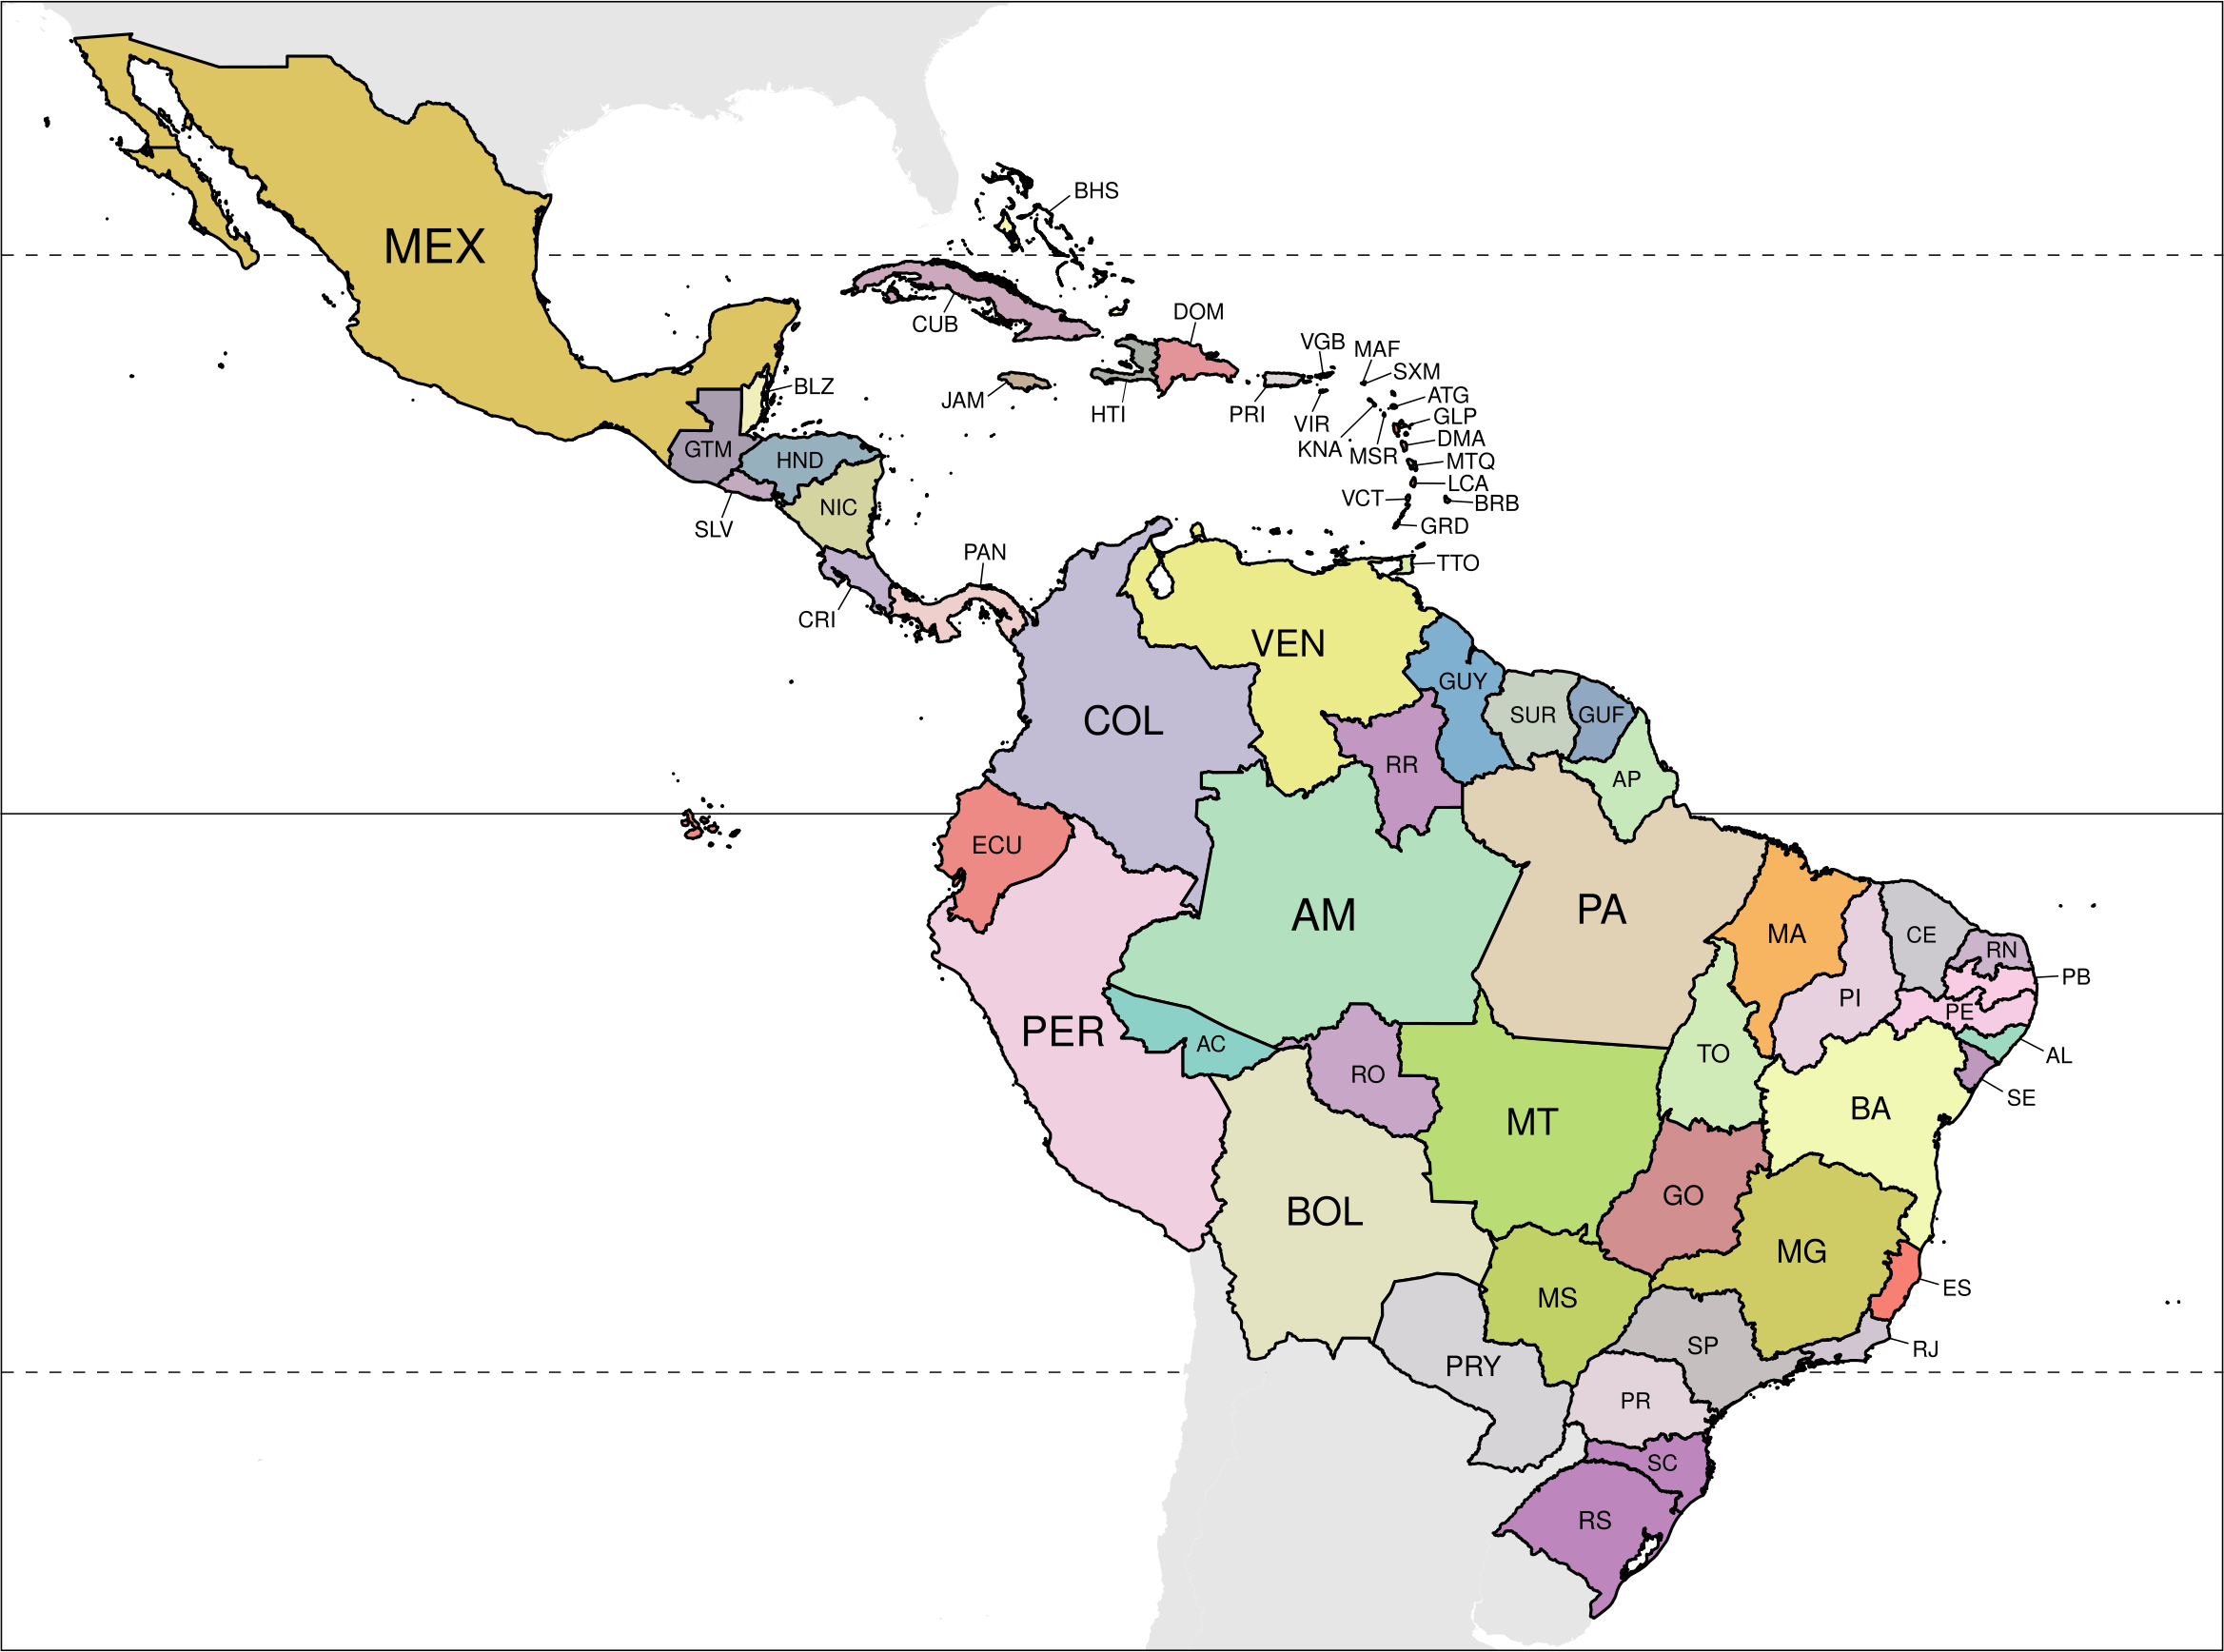
\includegraphics[width=0.32\textwidth]{figs/sm/study_areas_America}
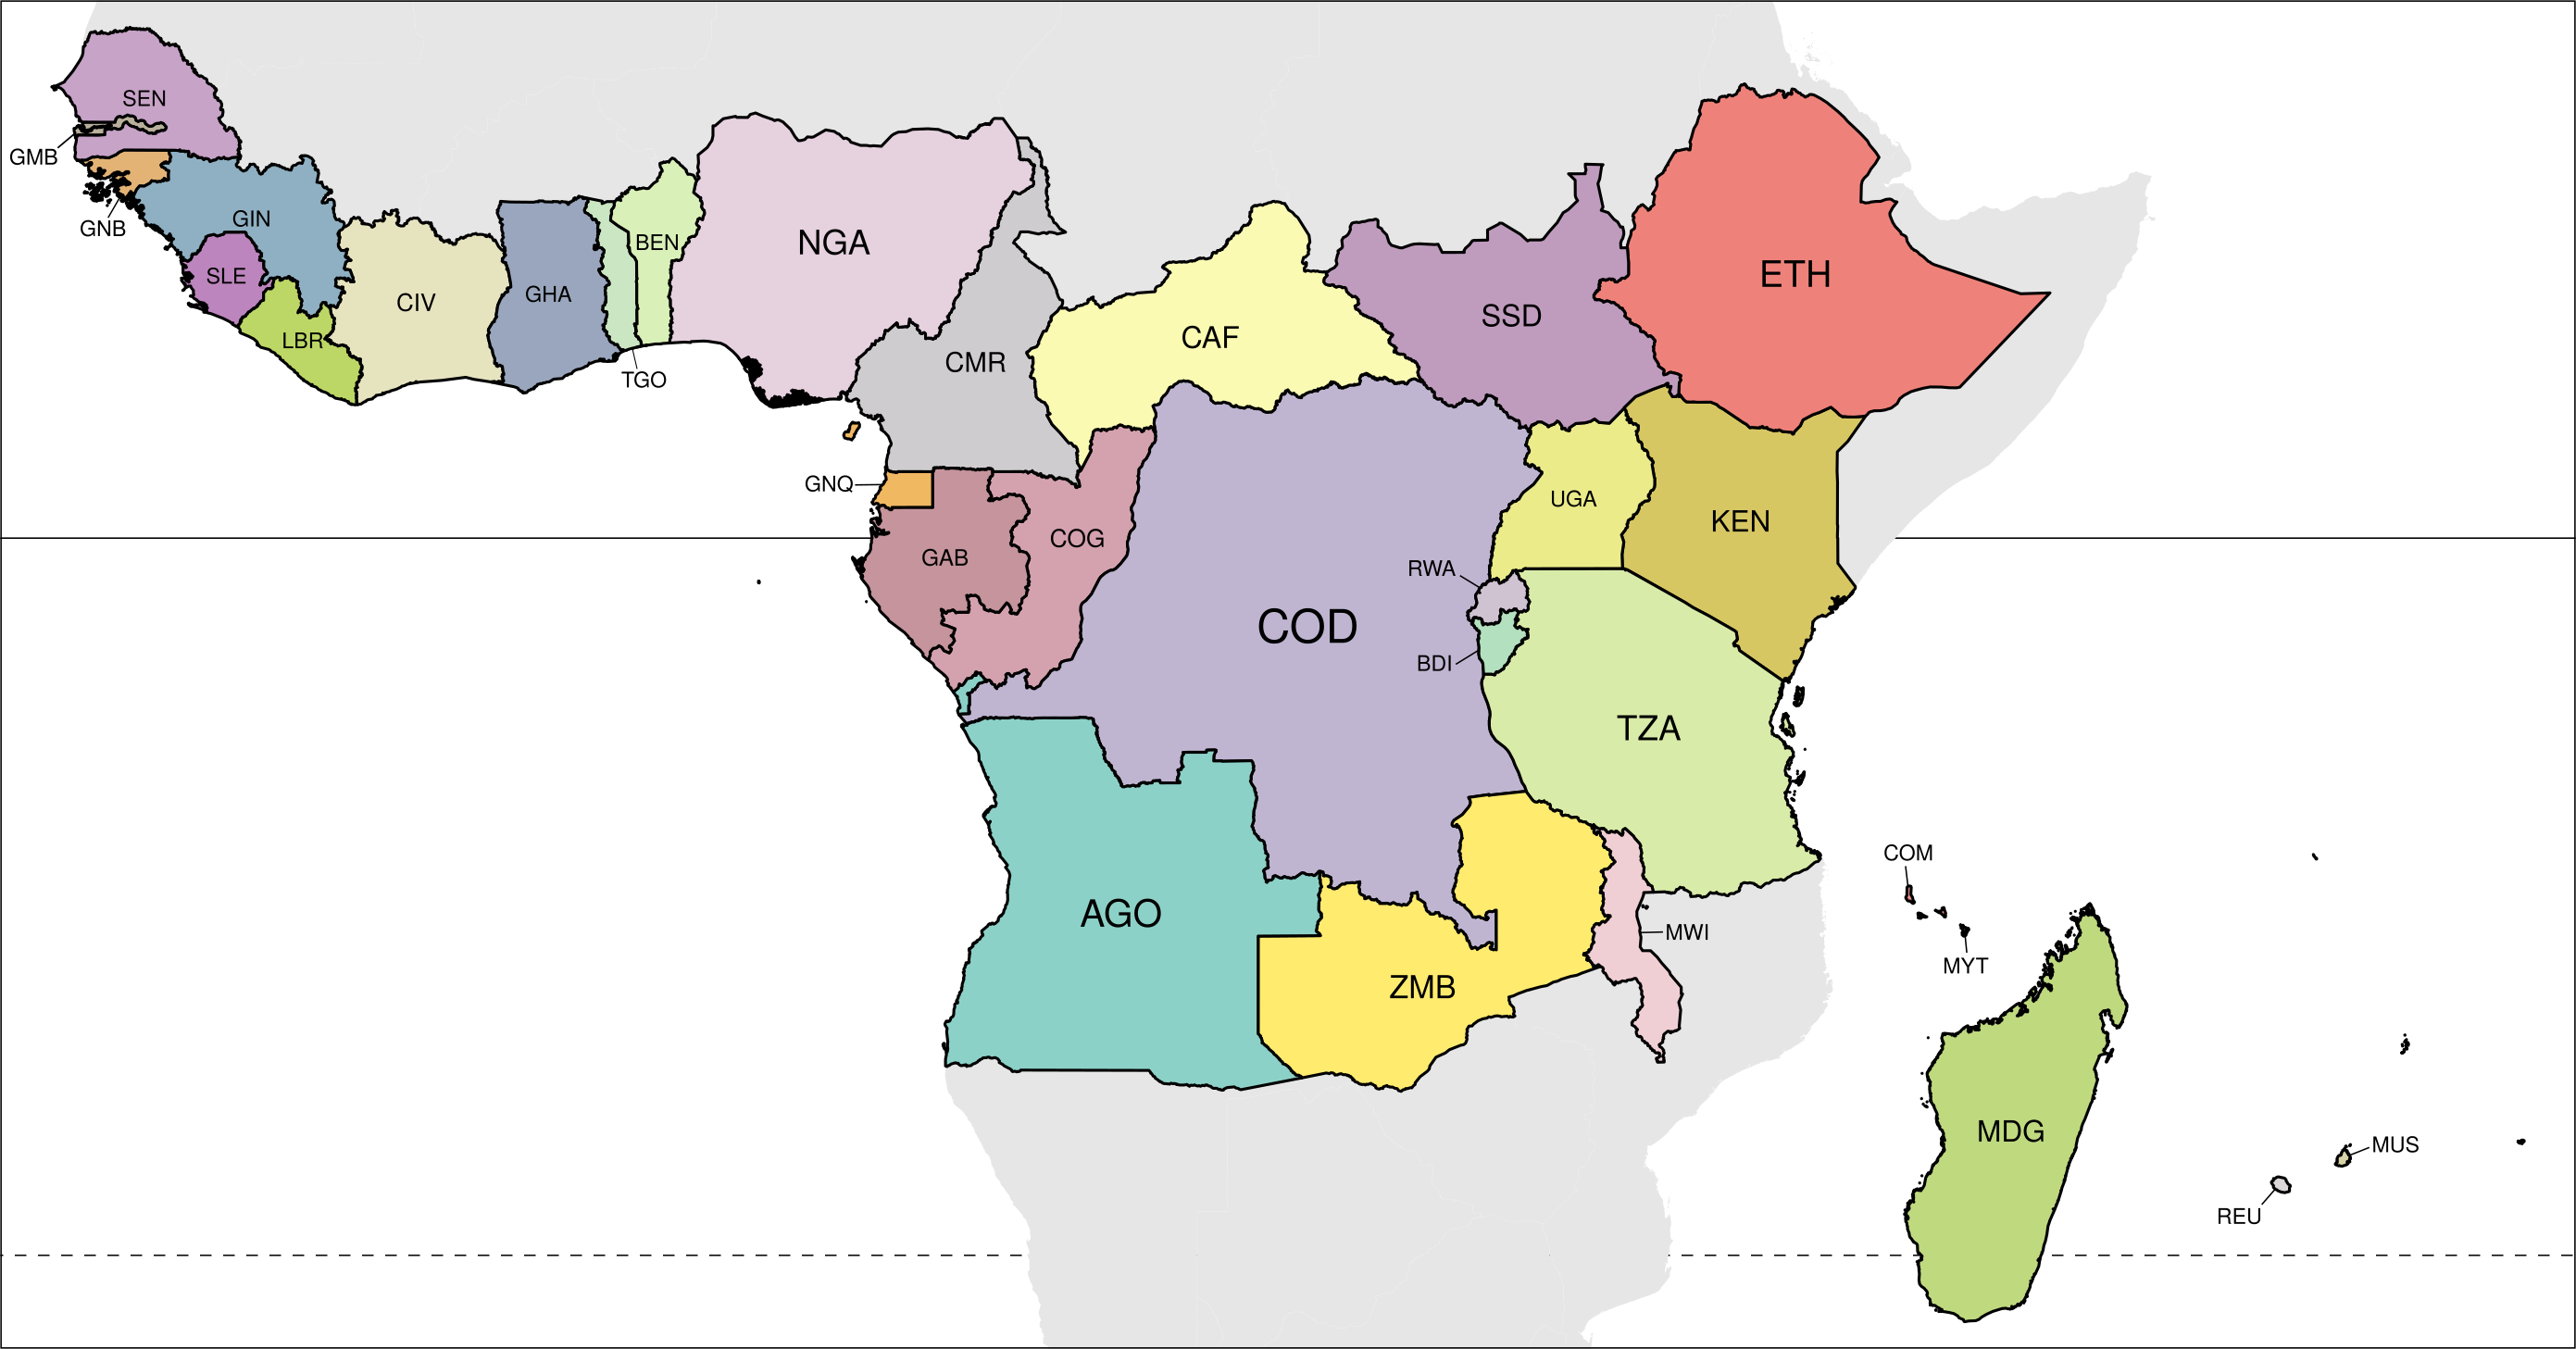
\includegraphics[width=0.32\textwidth]{figs/sm/study_areas_Africa}
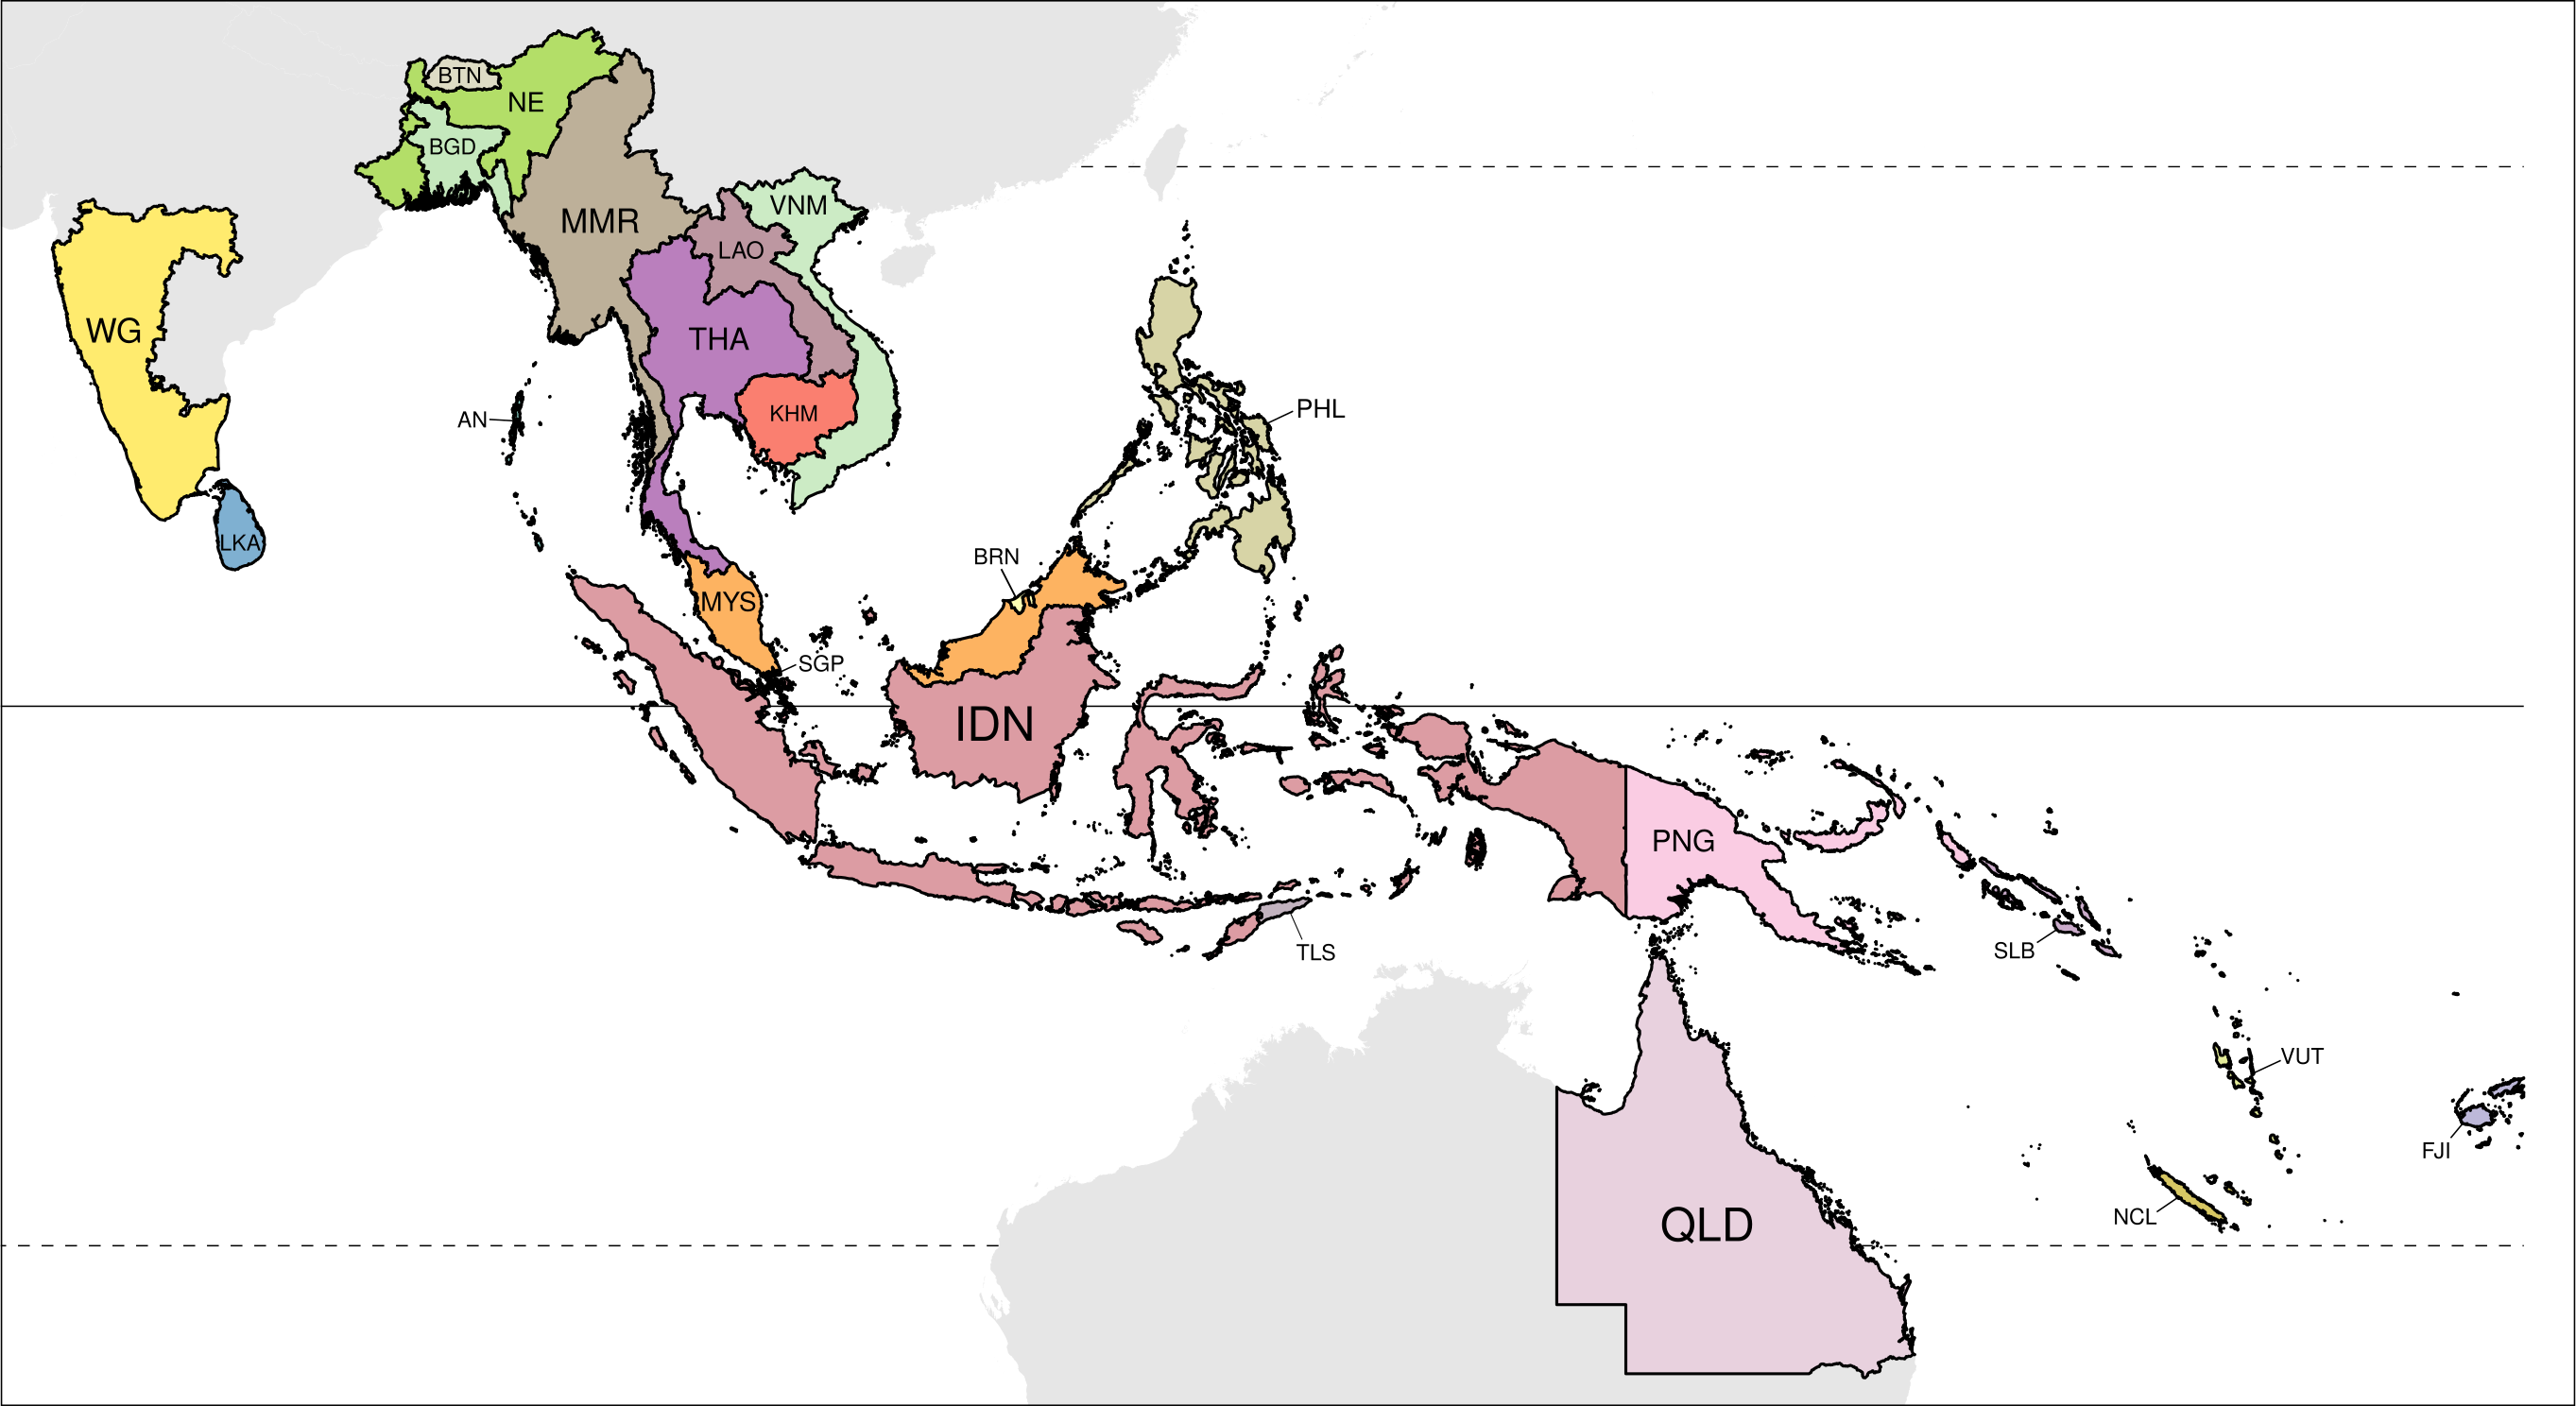
\includegraphics[width=0.32\textwidth]{figs/sm/study_areas_Asia}
\textbf{The 119 study areas in the 3 continents}
\end{center}
\end{frame}

\begin{frame}[label={sec:org2dafe56}]{ForestAtRisk in the tropics}
\begin{center}
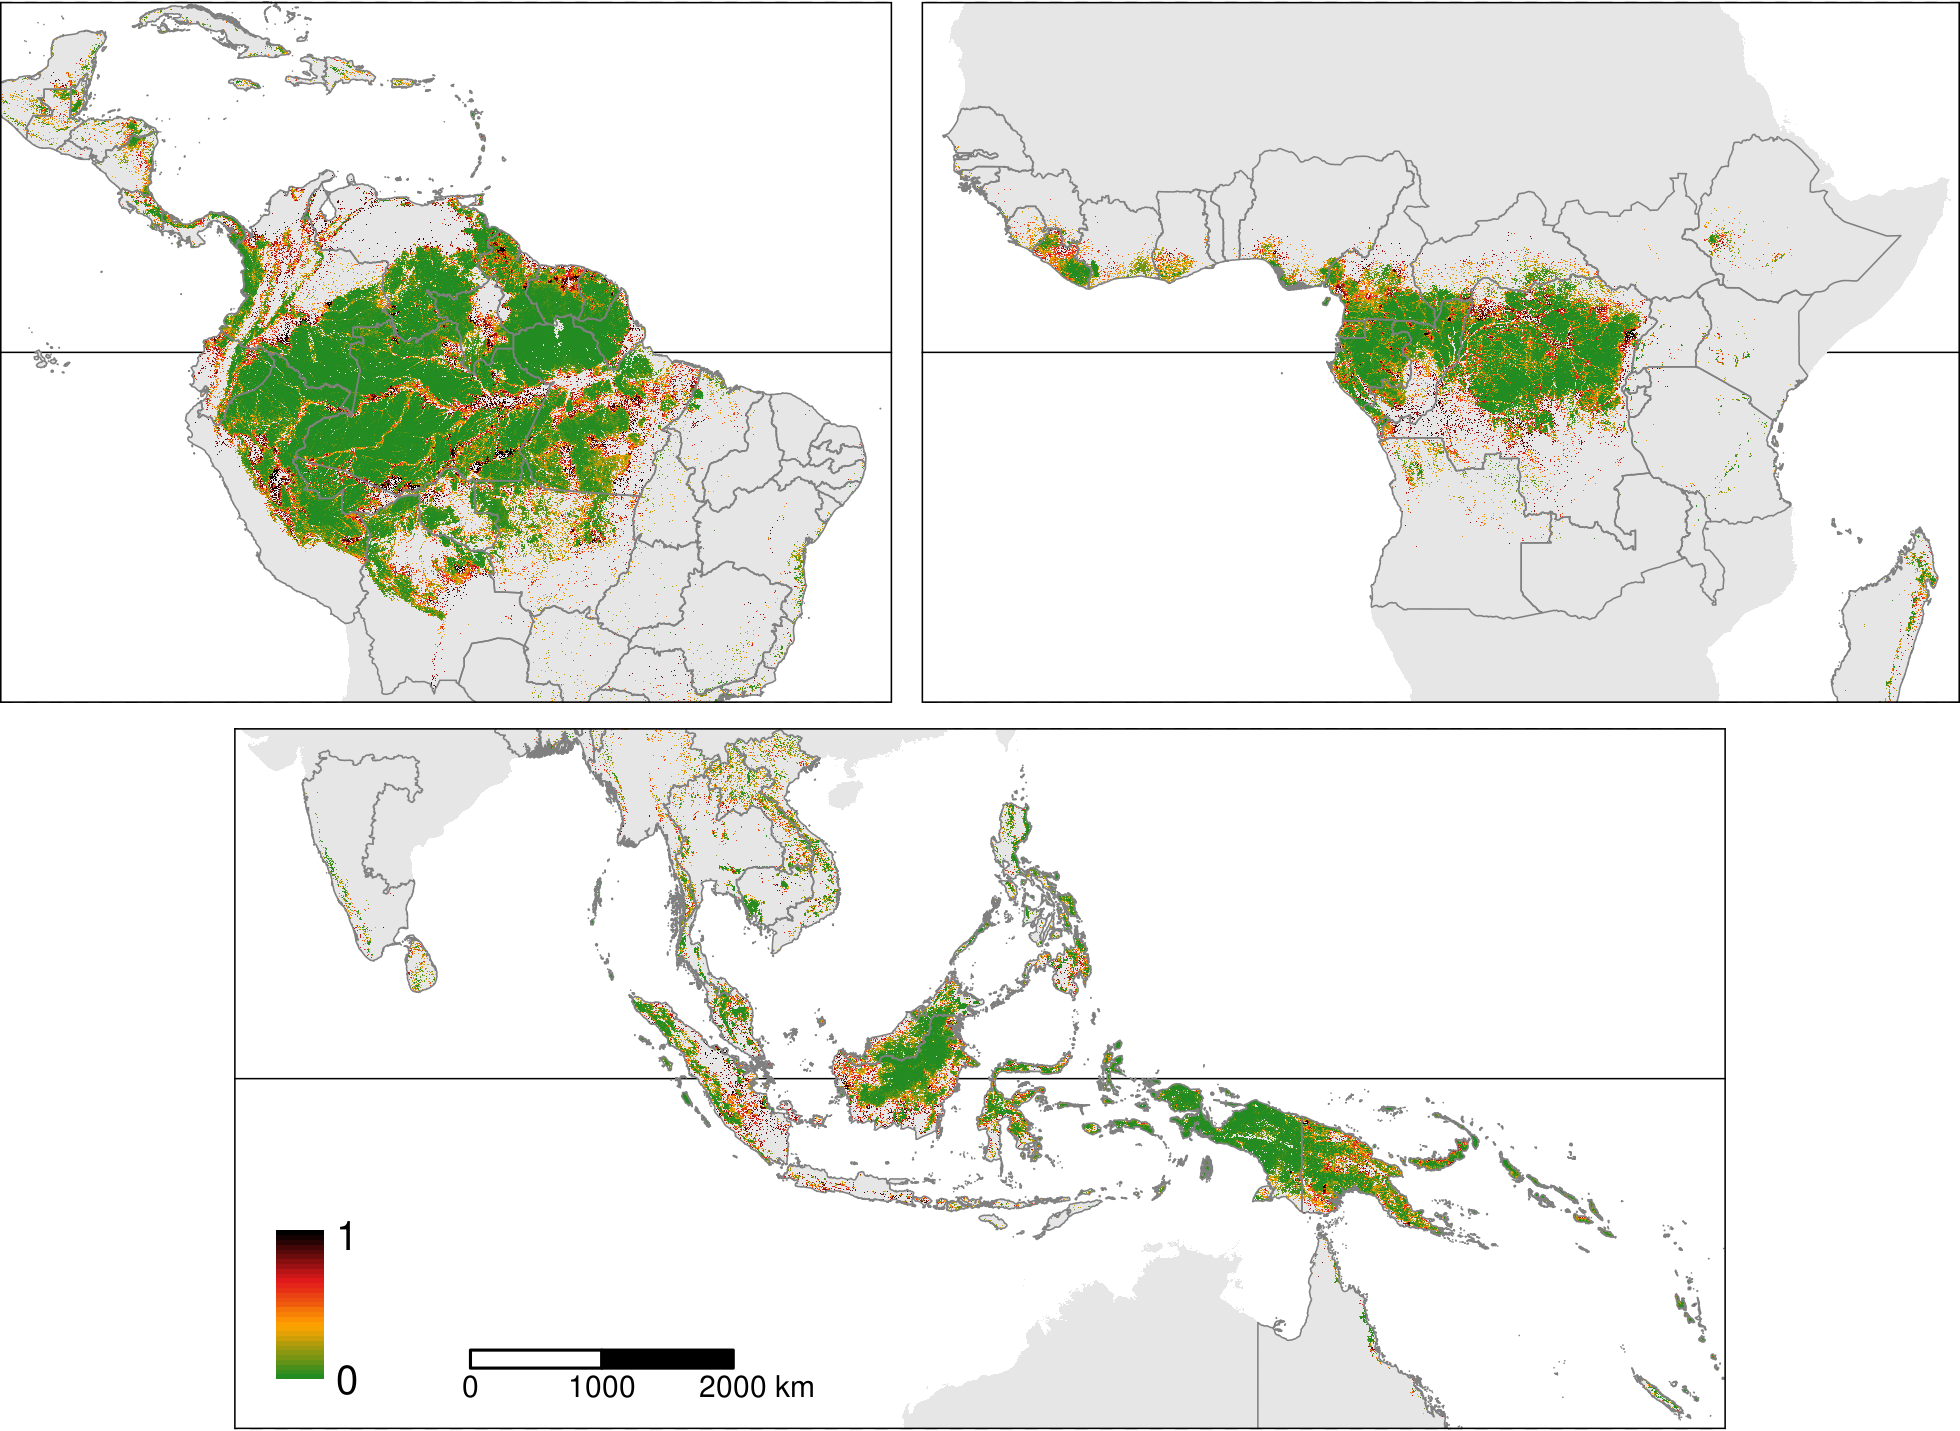
\includegraphics[width=0.7\textwidth]{figs/article/prob.png}
\end{center}

\textbf{Pantropical map of the spatial probability of deforestation}

Article in review: \href{https://doi.org/10.1101/2022.03.22.485306}{10.1101/2022.03.22.485306}

\url{https://forestatrisk.cirad.fr/maps.html}
\end{frame}

\subsection{Moving window models}
\label{sec:org40ee9dc}

\begin{frame}[label={sec:org25eb7c1}]{Moving window models}
\end{frame}

\section{Usage}
\label{sec:org94ce2c4}

\subsection{Allocating deforestation}
\label{sec:org159daca}

\begin{frame}[label={sec:orgb0ea3a5}]{Allocating deforestation}
\end{frame}

\subsection{Subnational jurisdictions}
\label{sec:org7f33d2f}

\begin{frame}[label={sec:orgd839180}]{Subnational jurisdictions}
\end{frame}

\subsection{User's data}
\label{sec:org2337ee1}

\begin{frame}[label={sec:org00152ad}]{User's data}
\end{frame}

\section{Conclusion}
\label{sec:orga9b4560}

\subsection{Week agenda}
\label{sec:org822e37d}

\begin{frame}[label={sec:org4be7945}]{Week agenda}
\end{frame}

\subsection{Perspectives}
\label{sec:org9e9a308}

\begin{frame}[label={sec:org967046d}]{Perspectives}
\begin{itemize}
\item Increase computational speed (for predictions on large areas).
\item Adding more alternative models (MLP).
\end{itemize}
\end{frame}

% %%%%%%%%%%%%%%%%%%%%%%%%%%%%%%%%%%%%%%%%%%%%%%%%%%%%%%%%%%

{
  % Use background image
  \usebackgroundtemplate{%
    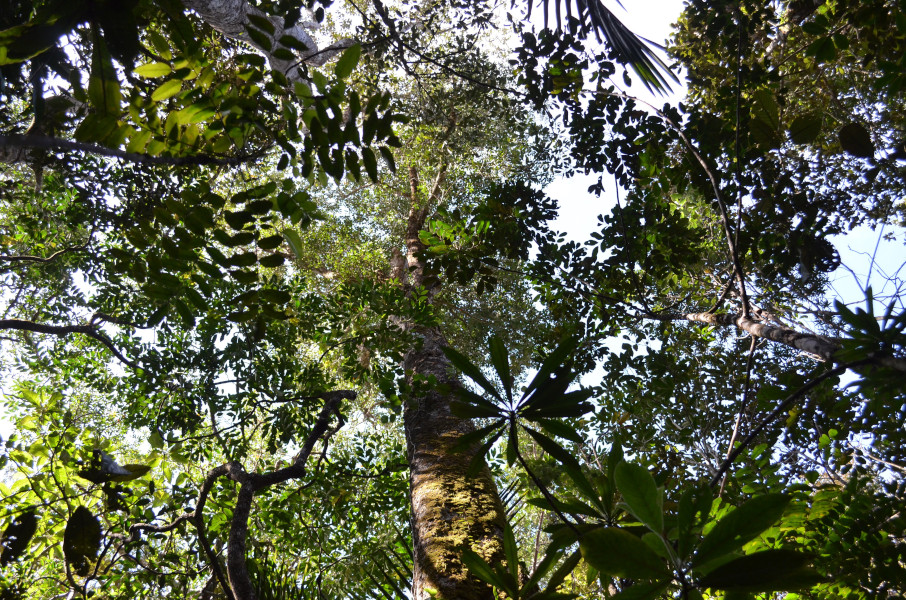
\includegraphics[keepaspectratio=true, height=\paperheight]{figs/Canopy-NC}
  }
  \setbeamertemplate{navigation symbols}{}
  % Remove shadow from block
  \setbeamertemplate{blocks}[rounded][shadow=false]
  \begin{frame}[plain]
  	\vspace*{\stretch{100}} 
    \begin{block}{}
      \begin{center}
        \ldots~Thank you for attention~\ldots \\
        \url{https://deforisk-qgis-plugin.org} \\
        \textbf{> Articles > References > Presentations} \\
        
\includegraphics[width=0.8\textwidth]{figs/partners_logos}
      \end{center}
    \end{block}
  \end{frame}
}
\end{document}
